\documentclass[../dejiny-rodu-prusiku.tex]{subfiles}

\begin{document}

% str 1 @ 2
\chapter{Prolog}

% TODO přepsat

% str 0+2(=1+1) @ 3

\section{Motto}

\renewcommand{\poemtoc}{subsection}
\poemtitle{Život}
\settowidth{\versewidth}{Smrt má tě za blázna, nebo klopotně}
\begin{verse}[\versewidth]
Jist buďte smrtí: potom smrt i život \\
vám budou sladší. Se svým životem \\
tak rozumujte: pozbudu-li tě, \\
tož pozbudu, co pošetilec jen \\
rád uchová: jsi dech a podroben \\
všem povětrným vlivům, kterými \\
tvůj byt je každou chvíli ohrožen. \\
Smrt má tě za blázna, nebo klopotně \\
jí ubíhaje, stále pádíš za ní.

\attrib{William Shakespeare}
\end{verse}

\renewcommand{\poemtoc}{subsection}
\poemtitle{Domovina}
\settowidth{\versewidth}{Mám rád nade všecko pravé lidské štěstí,}
\begin{verse}[\versewidth]
Mám rád nade všecko pravé lidské štěstí, \\
které musí dopřát člověk stejně všem. \\
Mám rád kameny i čerstvé ratolesti, \\
nade všecko miluji svou rodnou zem. \\
Nade všecko miluji svou malou ves. \\
Má ji každý člověk, ať je odkudkoli. \\
Nechat si ji urvat někým, strašně bolí. \\
Žíti bez vlasti je žíti hůř než pes.

Malé, nejmenší i velké národy, \\
máme všichni stejné závazky a práva, \\
psaná přísným prstem větru na vody, \\
na prapory států, jimiž lidstvo mává, \\
právo rozhodovat jménem většiny \\
rodným jazykem a ve své rodné zemi \\
o tom, co je stejně milováno všemi, \\
o štěstí a osudech své otčiny.

\attrib{Vítězslav Nezval}
\end{verse}

% str 2 @ 4

\section{Kolébka rodu}

Je začátek šestnáctého století, píše se rok 1515. Ve Francii nastupuje na trůn král František I., který později zve k sobě Leonarda da Vinci. V Anglii kraluje velký despota Jindřich VIII. Ve Španělsku vládne v dobách veliké inkvisice císař Karel I. A v Rusku utužuje svou svrchovanost otec Ivana Hrozného, Vasil III. V Čechách pomalu doznívá kralování Vladislava Jagelonského.

V malé západočeské vesničce, které říká lid Sedlice, rodí se první náš známý předek Vojtěch Prusík. Vesnice Sedlec, jak se úředně nazývá, leží na sever od Plzně, blíže starobylých Plas. Prvně se připomíná v historii r. 1193. Byla tehdy majetkem vladyky Humpolta z Pot­vorova, který ji odkázal klášteru v Plasích. V rukou plasských cisterciáků však Sedlec nebyl dlouho, neboť v roce 1250 není již v soupise majetku kláštera Plasy, ale obec drží rod pánů Hrabišiců, z nichž někteří byli v~přímých službách knížecích.

Za poručnické vlády Oty Braniborského v r. 1281 věnovali Hrabišici Kojata a Všebor tuto vesničku klášteru Křižovníků božího hrobu na Zderaze v Praze. Asi 120 let patři­la obec Sedlec tomuto klášteru, který byl v husitských bouřích zničen. Od roku 1421 byl majitelem Sedlce Hanuš Kolovrat z Krašova a po něm až do r. 1485 Kolovrat, křest­ním jménem Albrecht. Po roce 1485 až do roku 1529 byl majitelem obce Jetřich Bezdružický z Kolovrat. Od toho roku byl pak majitelem Mikuláš Sviták z Landštejna, jeho bratr Vilém a po něm Kateřina Svitáková ze Solopysk.

Od roku 1546 byli držiteli prasídla našeho rodu Gryspekové. Za tohoto rodu se nejvíce dovídáme o našich předcích. Prvním majitelem byl Florián Gryspek s Gryspachu, sekretář císa­ře Ferdinanda I. Florián vystavěl nádherný renesanční zámek na Kaceřově a nebyl-li zrovna v Praze u dvora či v ci­zině za úředním posláním, nejraději žil na Kaceřově. Mezi českou šlechtou Gryspek, původem Němec z Tyrol, nebyl oblí­ben, ale lid jej měl rád. Za Gryspeků se poddaným podle historického svědectví dařilo poměrně dobře. V urbáři, kte­rý založil pro pořádek na svém panství v r. 1558, je zmínka o našem předku Vojtěchu Prusíkovi.

Po bitvě na Bílé Hoře byl celý majetek Gryspeků zkonfiskován r. 1623 a odevzdán klášteru v~Plasích. V majetku toho­to mocného kláštera zůstal Sedlec až do zrušení jeho v r. 1785 císařem Josefem II.

Od Náboženského fondu koupil panství Plasy a tím i poddané Sedlce kníže Klement Metternich v~r.~1826.

V západní části obce, která je přivtělena farností k Potvorovu, je usedlost, která do r. 1805 měla číslo 9. Od toho roku až dodnes má č. 4. V tomto gruntě žil náš rod od nepaměti, prokazatelně však od roku 1515.

% str 2+1 @ 5

\begin{figure}
\centering
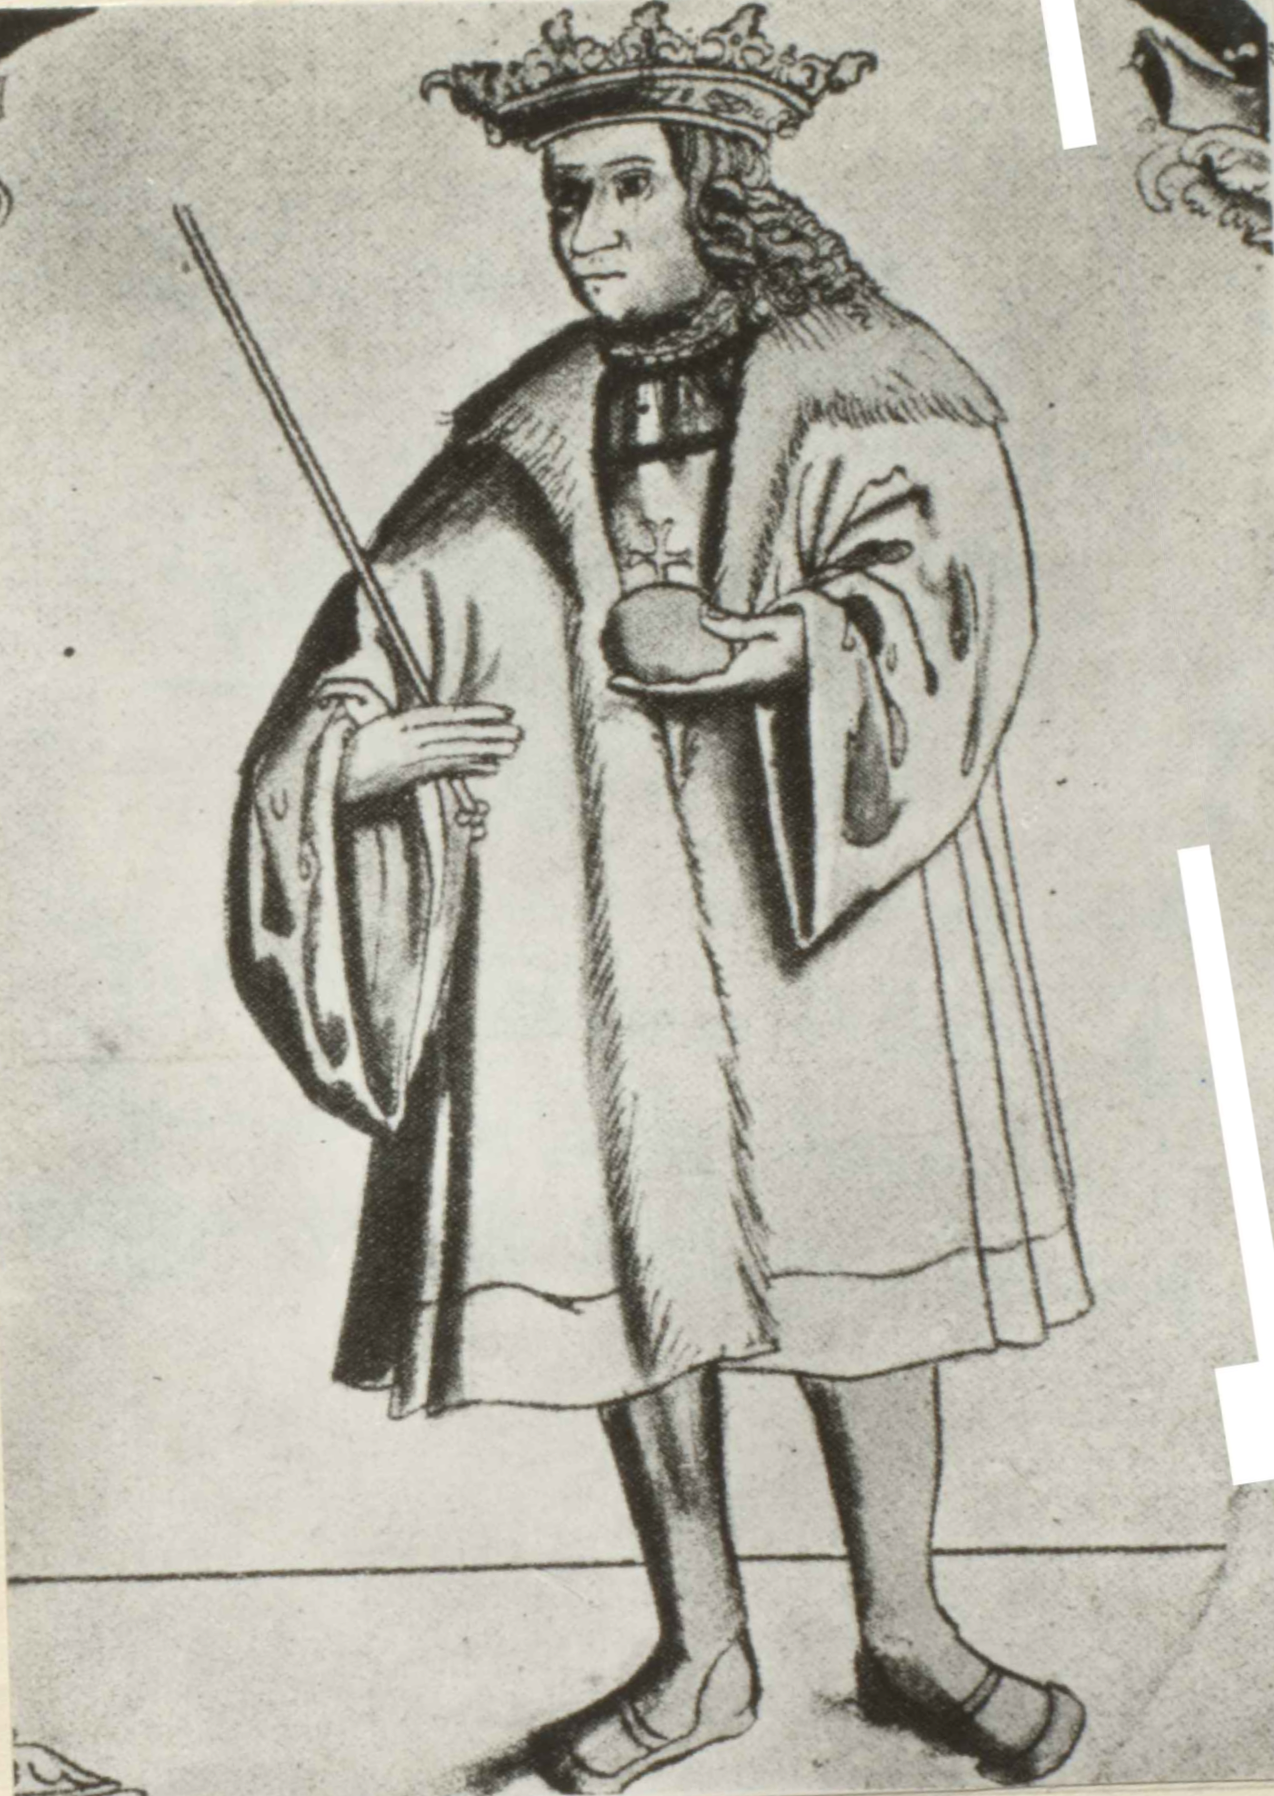
\includegraphics[width=\textwidth, height=\textheight, keepaspectratio]{005-a-vladislav_jagellonsky}
\caption{Český král Vladislav Jagellonský, za jehož panování (1491 – 1516) žil v Sedlci první náš známý předek Vojtěch Prusík}
\label{fig:005-a-vladislav_jagellonsky}
\end{figure}

% str 3 @ 6
Grunt č. 4 v Sedlci měl původně 2 lány půdy tj. asi dnešních 40 ha. Zahrada u statku nebyla přímo, ale napro­ti přes silnici. Náš rod vymřel po meči v tomto prasídle 14. června 1846, ale ještě dnes po tak dlouhých letech se tam říká "U Prusíků“. Tradice má opravdu hluboké ko­řeny. Rod Prusíků trvá dál v jiných vesnicích, krajích a zemích.

Sedlec leží uprostřed polí a luk, lesy nejsou u vesnice. Proto asi obec byla od pradávna osídlena, neboť pozemky byly již dávno kultivovány. Kdy přišli Prusíci poprvé do této obce, není známo. Panují jen legendy o původu našeho jména přenášené ústním podáním v rodě z generace na genera­ci.

V roce 1039 za rozháraných poměrů po smrti Boleslava Chrabrého v Polsku vtrhl do této země český kníže Břeti­slav I. Dobyl četná města a mimo jiné i opevněné město Gdecz. Z Hnězdna přivezl do Čech ostatky sv. Vojtěcha. Kromě velké kořisti přivedl domů i značný počet zajatců, kterým však dal později všechna práva a usadil je v růz­ných západočeských krajích, zvláště také na Kralovicku.

Zde je obec Hedčany a Hedečko, zbytky bývalého velkého Újezdu hedčanského. Za krále Václava I. se Újezd rozpadl a svobodní potomci Poláků a Prusů se rozešli po kraji. Snad náš předek patřil k~nim. Jiný původ našeho jména a rodu je však také možný, ale nějakou souvislost s bývalý­mi Prusy v Pobaltí máme. Vzhledem k tomu, že asi o 80 let dříve než se narodil Vojtěch Prusík, tedy v~polovině XV.~století, začínali se lidé pojmenovávati přesně příjmením, je také možné, že některý náš předek táhl do Polska a pohanských Prus a po návratu pak dostal jméno Prusík. Takových českých válečných výprav bylo v historii mnoho. Již sv. Vojtěch působil v Prusích v X. století, pak byli Češi v Prusích za krále Přemysla Otakara II, Jana Lucemburského a také v XV. století za dob husitských. Vždyť Jan Čapek ze Sán, v jehož průvodě byl i hejtman Jan z Královic, vstoupil v~r.~1433 až do vod Baltu a odtud do vlasti si se svými druhy přinesl mořskou vodu na památ­ku. Jak jsme přišli ke jménu, může být i tento výklad pravděpodobný. Nejblíže pravdě však asi bude, že naši před­ci ještě před 16. stoletím, před 1000 lety žili blízko Prus v dnešním severním Polsku. O tom však později. První náš předek je psán tak, jak my se dnes píšeme, ale průběhem staletí mnohdy se psávali naši předci jako Prusyk i Prussik. Dnes se píší všichni u nás jako Prusík s čárkou a v cizině s tečkou na i. Jen jeden člen rodu v naší historii změnil jméno na Prusek. Žije v USA.

% str 3+1 @ 7
\begin{figure}
\centering
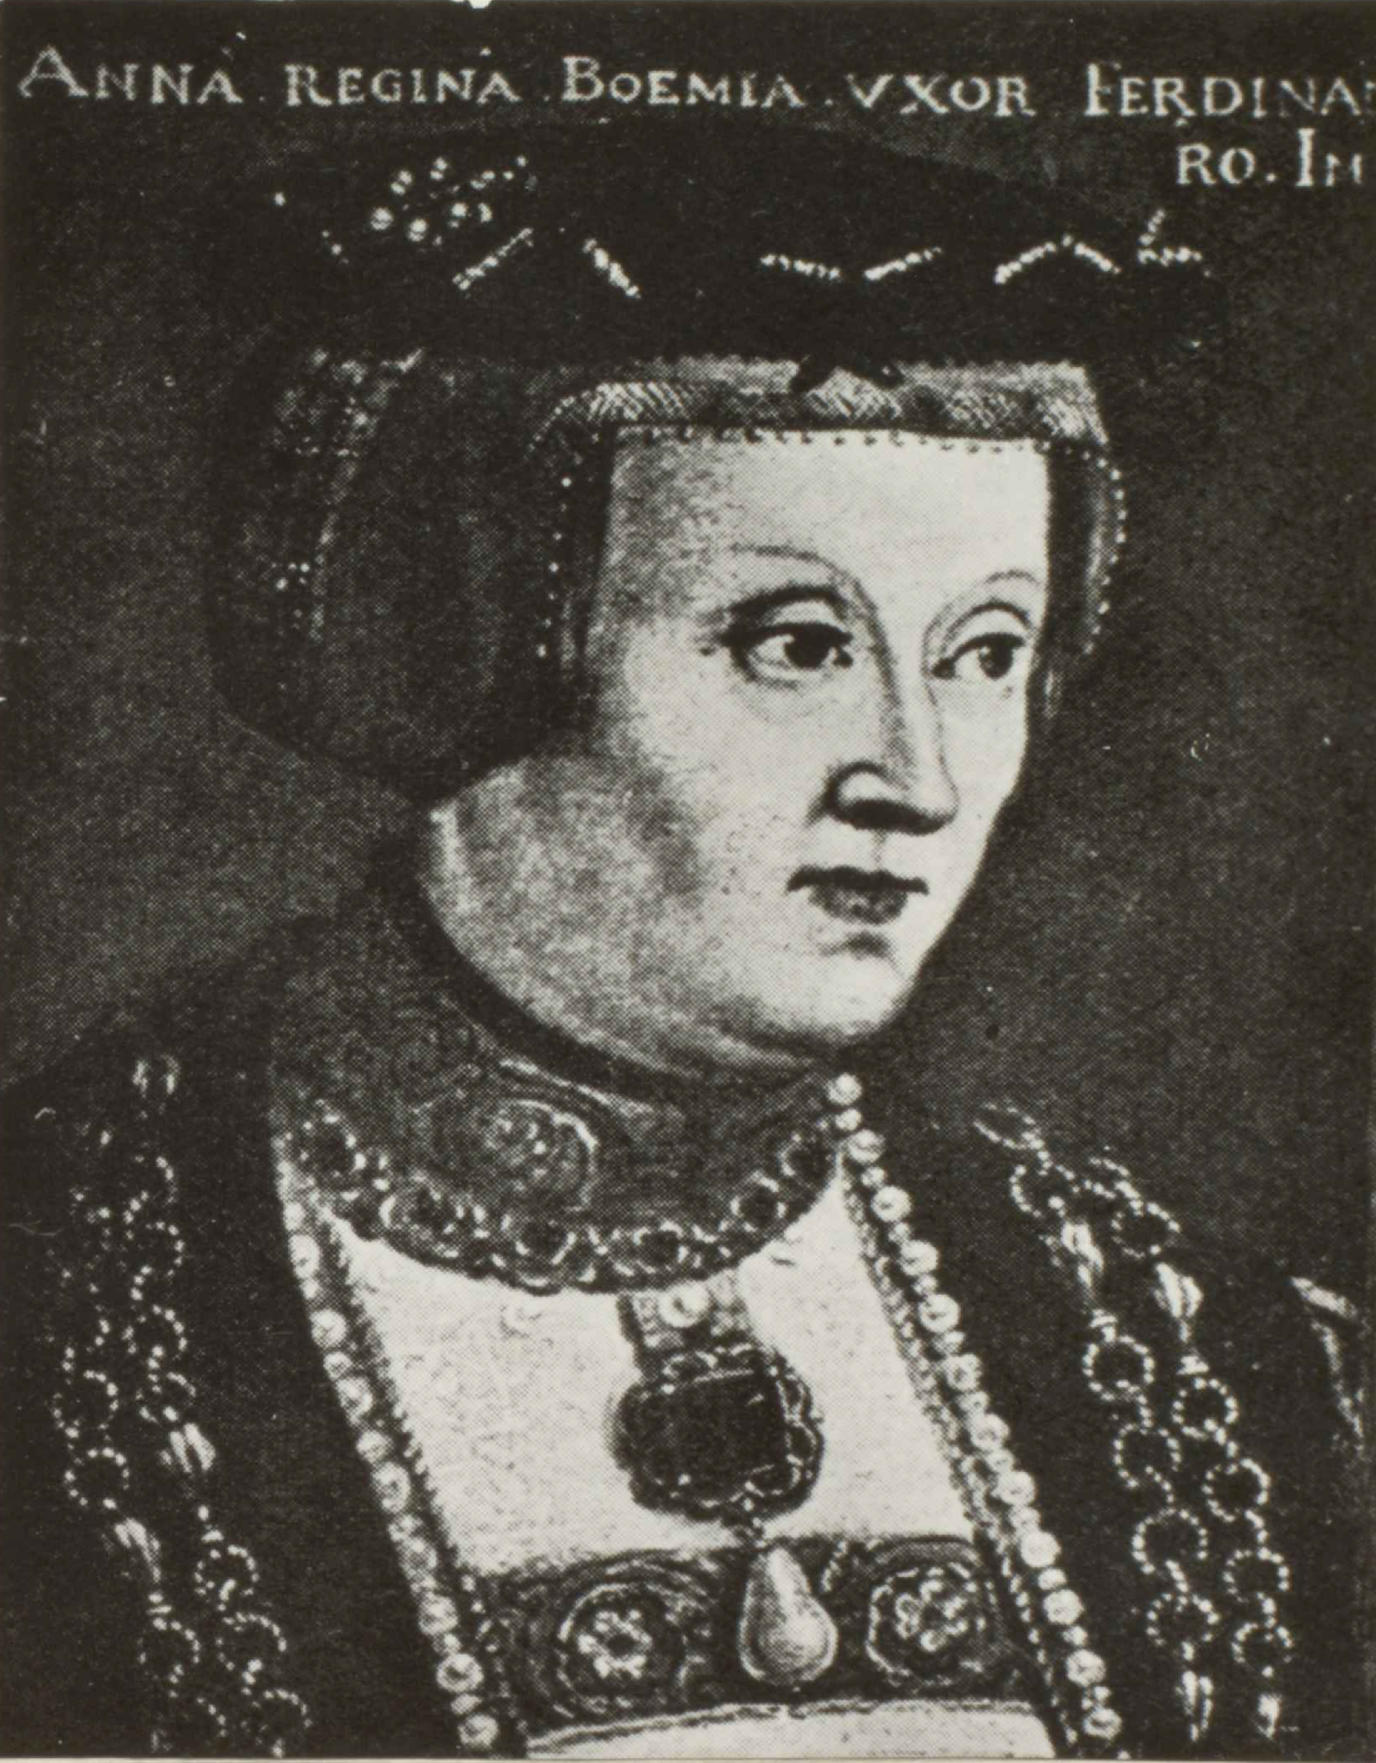
\includegraphics[width=\textwidth, height=\textheight, keepaspectratio]{007-a-anna_jagellonska}
\caption{Anna Jagellonská, manželka prvního Habsburka na českém trůně; za jejího panování hospodařil v Sedlci  náš dávný předek Vojtěch Prusík (1515 – 1580)}
\label{fig: 007-a-anna_jagellonska}
\end{figure}


% str 4 @ 8
V první polovině XVI. století bylo v Sedlci 8 lidí "osedlých". Jmenovali se Havel Levý, Vaněk Bureš, Mika Jakeš, Jan Polívka, Blažej Jánský, Simon Brož, Jan Bavor a největší hospodář Vojtěch Prusík. Celkem měli tito usedlíci tehdy 10 lánů půdy. Na každý lán připadal plat po dvou slepicích, deseti vejcích, o sv. Jiří jedna ko­pa a osm grošů, o Havlu jedna kopa a šest grošů. Simon Bureš měl velkou zahradu a proto platil z ní o pololetí o dvacet grošů více. Dohromady platili usedlíci ze Sedl­ce Gryspekům na zámek Kačerov svatojirského úroku jedenáct kop a čtyřicet grošů, havelského úroku 11 kop a dvacet grošů, dvacet úročních slepic a jednu kopu a čtyřicet vajec na velikonoce.

Usedlost Prusíků byla poměrně velká a ještě v roce 1962 existovala u statku starobylá dřevená stodola, která by­la postavena nedlouho po třicetileté válce. Číslo 4 v Sedlci u Potvorova je nejstarší známá kolébka našeho ro­du. Veliký počet členů rodu neví již pranic o tomto svém prasídle, ani o svých dávných předcích, kteří se zde na­rodili, odtud vyšli do světa, založili rodové větve a jejich potomci žili pak a žijí v jiných koutech naší vlasti i daleko v cizině a za mořem. Osvětlíme si v tomto vyprávění dávnou dobu i lidi, k nimž pokrevně patříme ja­ko jejich potomci.

Zlé i dobré časy přeletěly nad naší zemí, generace se vystřídaly s generacemi a mnoho přerůzných osudů prožil náš rod. Dějiny Prusíků započínáme proto prvním, historicky zjištěným předkem naším, sedlákem Vojtěchem Prusíkem ze Sedlce.

Společný předek nás všech  Vojtěch  Prusík  narodil se v r. 1515, rok před smrtí krále Vladislava Jagelonského. O jeho otci není nám nic známo. Vojtěch převážně hospodařil již za Gryspeků a jako rychtář musil se často objevovat na zámku Kaceřově. Tam odváděl plat za držení všech usedlostí v~obci, ale roboty tehdy nekonal nikdo. Povinnosti byly jen platební a byly přesně vymezeny v urbáři kaceřovském, který byl sepsán v červnu a ukončen v neděli po sv. Trojici v r. 1558. Vojtěch měl za ženu Voršilu Rajskou, ale odkud pocháze­la a kdy zemřela nepodařilo se zjistit. Z jeho dětí je znám pouze syn Mikuláš, dědic gruntu. Vojtěch Prusík, jakási legendární postava našeho rodu, zemřel v~Sedlci v roce 1580.

Vojtěchův syn, Mikuláš Prusík, narodil se roku 1550. Své jméno dostal patrně po patronu kostela sv. Mikuláše v~Potvorově, kde byl pokřtěn jako všichni naši předci před ním i po něm, kteří žili v~Sedlci. Mikuláš zemřel na počátku třicetileté války v r. 1625. Hospodařil na gruntě v dobách císaře Rudolfa II.

% str 4+1 @ 9

\begin{figure}
\centering
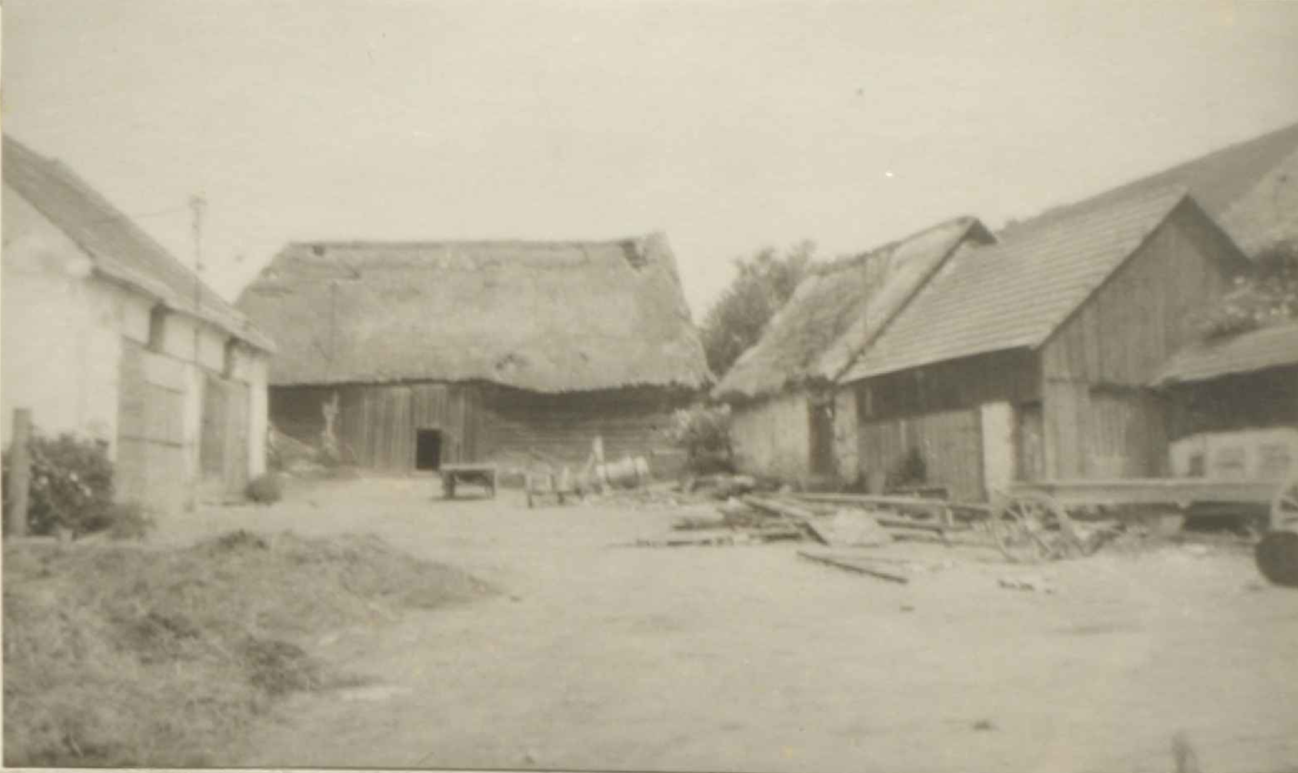
\includegraphics[width=\textwidth, height=\textheight, keepaspectratio]{009-a-zbytky_gruntu}
\caption{Pohled na zbytky gruntu v Sedlci č. 4, kde stála první kolébka rodu. Stodola, která existovala do roku 1962, byla vystavěna po třicetileté válce}
\label{fig: 009-a-zbytky_gruntu}
\end{figure}

\begin{figure}
\centering
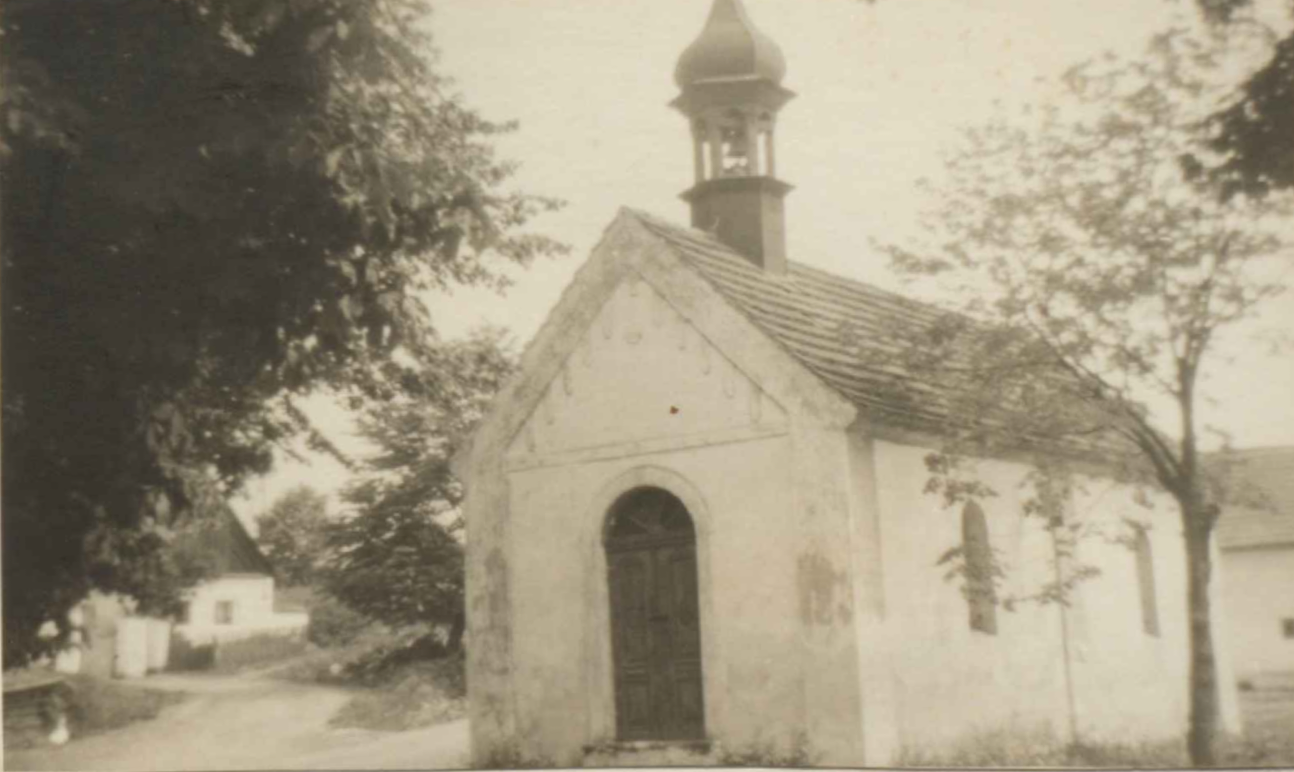
\includegraphics[width=\textwidth, height=\textheight, keepaspectratio]{009-b-kaplicka_v_sedlci}
\caption{Kaplička na návsi v Sedlci}
\label{fig: 009-b-kaplicka_v_sedlci}
\end{figure}


% str 5 @ 10

Synem Mikulášovým byl Václav Prusík. Narodil se roku 1580 a podle urbáře kláštera v Plasích hospodařil v r. 1623 tehdy v těžké době pobělohorské, v prasídle našeho rodu. Ve starých listinách je psán jako Prusyk, ačkoliv jeho dědeček Vojtěch je psán správně jako první Prusík a většina dalších členů rodu. Václav zemřel ještě před koncem třicetileté války v roce 1640. Z jeho dětí jsou známi dva synové. Starší byl Jakub, o rok mladší Bartoloměj.

Jakub Prusík dostal rodný grunt. Narodil se v roce 1601 a jeho ženou byla Anna nar. 1603, která přežila svého muže o jeden rok. Podle soupisu poddaných podle víry z roku 1651 žilo v Sedlci 32 obyvatel. Některé pustiny po třicetileté válce byly znovu osazeny, ale prusíkovský grunt, jak se zdá, nebyl valně poškozen. Jakub měl tři syny a jednu dceru. Nejstarší byl Matouš, který se na­rodil v~roce 1628. Přiženil se pak v roce 1650 do Bílova k Rejčkům a žil až do roku 1696. Potomci se jménem Prusík po něm nezůstali. Jakub Prusík zemřel roku 1672. Manželka Jakuba Prusíka Anna narozená v roce 1605 byla rozená Hynková z Bílova u Kralovic.

Druhý syn Jakubův byl Václav Prusík. Narodil se o dva roky později roku 1630, stal se kovářem a usa­dil se v Bílově. Podle historie byl to velmi silný muž, často obhajoval zájmy lidu v různých půtkách s vrchností a jedno takové střetnutí se mu stalo nakonec osudné. Obyvatelé z Lednice se několik let přeli o louky se šlech­ticem Norbertem Miseronim, který byl majetnikem hradu Krašova. Když tyto spory vrcholily, povolali si lednič­tí kováře Václava Prusíka na pomoc a v půtce byl Václav tímto tyranským šlechticem 11. dubna 1673 zastřelen. Ně­kolik let potom v r. 1680 vypuklo všeobecné selské povstá­ní vedené Jiřím Radimem ze Dřevce. Václavovou ženou byla Barbora, která ho přežila o řadu let a zemřela v Mladoticích. Potomci s naším jménem po něm nezůstali. Barbora byla rozená Juhová z Bílova.

Třetím synem Jakubovým byl Martin Prusík, který zůstal na rodném gruntě. Byl společným předkem všech Prusíků dnes žijících ve světě, kromě těch, kteří žijí v Polsku.

Sestrou těchto tří bratrů byla Anna Prusíková, která se narodila v roce 1647 a provdala se ke Kymlům čili ke Kouklům do Bílova. Zemřela tam v roce 1738.

Otec těchto čtyř dětí, Jakub Prusík, zemřel v roce 1672 v Sedlci a jeho žena Anna o rok později.

% str 5+1 @ 11

\begin{figure}
\centering
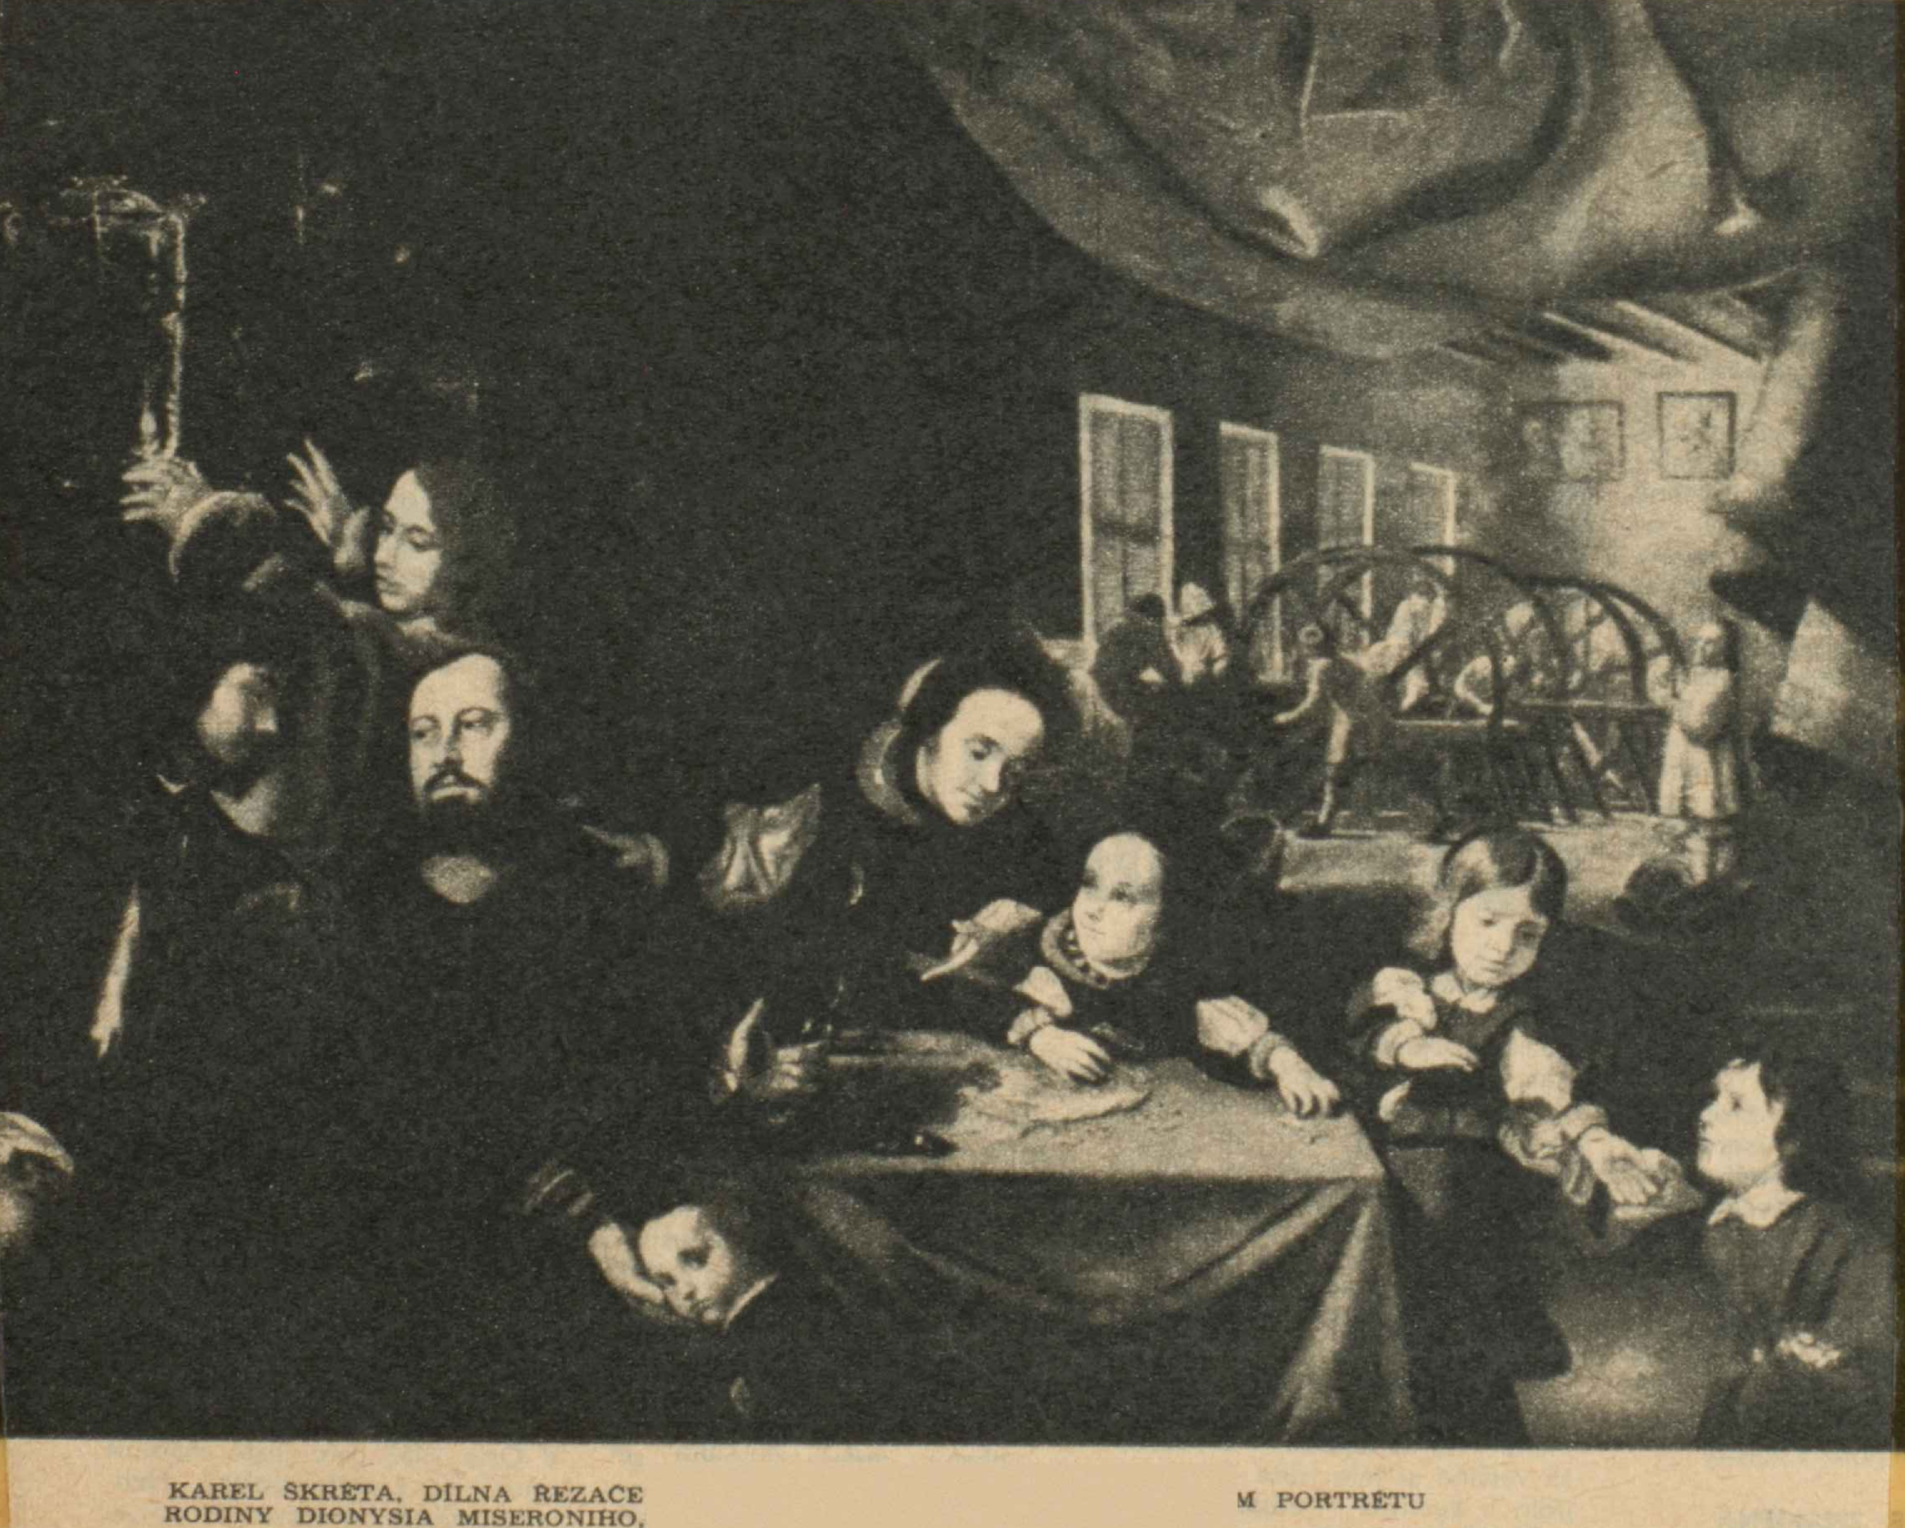
\includegraphics[width=\textwidth, height=\textheight, keepaspectratio]{011-norbert_miseroni}
\caption{Dítě v pravém rohu dole je pozdější majitel hradu Krašova Norbert Miseroni, vrah kováře Václava Prusíka z Bílova}
\label{fig:011-nobert_miseroni}
\end{figure}


% str 6 @ 12
Jakubův bratr Bartoloměj Prusík měl osudem předurčen pohnutý život. Narodil se v roce 1602 v Sedlci a když mu bylo 24 let, přiženil se v roce 1626 k mladé vdově po Pavlu Radimovi v Dřevci, který byl při kácení lesa zabit. Grunt to byl pěkný, měl dva lány a slušné stavení. O padesát let později žil v této usedlosti Jiří Chlupsa, řečený Radim, vůdce selského povstání. Dlouho však v Dřevci Bartoloměj se svou že­nou nežili. Když v roce 1627 za císaře Ferdinanda II. bylo vyhlášeno, že každý se musí státi katolíkem, ode­šlo z Čech mnoho protestantů a českých bratrů. I v Dřevci zůstal toho osudného roku jednou na podzim radimovský grunt pustý a nikdo dlouhá staletí o Barto­loměji Prusíkovi a jeho ženě již neslyšel. Po 340 letech po klikatých cestách světem našla se jeho stopa v Pol­sku. Když jsem hledal všechny Prusíky ve světě, nalezl jsem jednoho Matěje Prusíka, který pracoval jako bio­log na universitě v New Brunswick ve státě New Jersey, blíže New Yorku. Je polského původu a když se pátralo v Polsku po jeho předcích, došlo k velikému překvapení. Jeho dávným předkem, jako ostatních Prusíků v Polsku, je exulant Bartoloměj Prusík. Po strastiplné cestě Saskem dostal se Bartoloměj až do Ostrowa Mazowieckego na se­verovýchod od Varšavy a tam zemřel v roce 1670, kdy do­končil svou životní pouť ve vyhnanství Jan Amos Komen­ský.

V první polovině XVII. století žili Prusíci jen v Sedlci a exulant Bartoloměj Prusík se svými potomky v Polsku. Nikde jinde tehdy tento rod neexistoval. Šířil se pak dále v Polsku, Čechách, rozmnožoval se v Sedlci a odtud pak dále do jiných míst. Později pak také do ciziny ji­né než do Polska.

Synovec Bartolomějův a syn Jakuba Prusíka, Martin Pru­sík, který zůstal na gruntě v Sedlci, narodil se uprostřed třicetileté války v r. 1633. Krušné časy nastaly jako všude, tak i v této obci a byly tu spáleny v té době čty­ři statky. Náš rodný grunt, prakolébka rodu nepadl však ani ohni, ani ničivým živlům válečným za oběť.

Martin Prusík převzal statek po smrti své matky Anny, která zemřela začátkem roku 1673. Předání sta­lo se 23. února 1673 v Plasích. Za ženu vzal si Martin Ludmilu Burdovou z Potvorova, která se tam narodila v ro­ce 1656. Martin neprožil jen pohnuté doby třicetileté války, ale i selské povstání na Kralovicku r. 1680. Z jeho dětí dospěly pouze tři, dcera a dva synové. Ka­teřina narodila se v~r.~1664, takže Jakub s Annou mohli se ještě několik let těšit ze svého vnoučete. Provdala se pak za Bernarda Kymela (Koukla) do blízkého Bílova. Tam zemřela 2. června v roce 1744 ve věku 80 let. Syni Martina a Ludmily se narodili až po smrti dědečka Jaku­ba a babičky Anny. Starší byl Václav, který se narodil v roce 1678 a mladší Martin po otci, narozený 1680. Na výměnku žil Martin Prusík 10 let. Jeho žena ho předešla do hrobu o dva roky, zemřela 7. ledna 1721. Martin zemřel v~patriarchálním věku 90 let dne 13. srpna 1723.

% str 7 @ 13
Nejstarší syn Martinův Václav Prusík byl předurčen k jinému zaměstnání než selskému. Narodil se v roce 1678 a když mu bylo 22 let, odešel do Plas a tam se později stal hostinským. V roce 1713 se oženil jako první Prusík s Němkou Sabinou Kirchgangovou, dcerou klášterního kováře. Z jeho pozdějších potomků vynikli mnozí různým způsobem a stali se zakladateli několika rodových větví. Václav Prusík zemřel v Nebřežinech u Plas 28. listopadu 1728.

Mladší syn Martin Prusík narodil se v Sedlci roku 1680. Oženil se 17. října 1702 s Annou Šlachovou z Bílova, která byla o osm let starší než on. Dne 14. března 1713 převzal grunt. Když jeho žena zemřela 27. dubna 1722, oženil se podruhé 4. srpna téhož roku s dcerou kováře v Sedlci, Annou Janečkovou. Děti jeho, které dospěly, byly jen z prvého manželství, z druhého manželství narozené brzy zemřely. Martin měl tři dcery a jed­noho syna. Anna narodila se 3. dubna 1704 a provdala se pak k Masopustům do blízké obce Bukoviny. Další dcera Eva narodila se 7. března 1718 a provdala se k Hrdíkům do Potvorova. Třetí Veronika narozená v roce 1720 prov­dala se k~příbuzným své matky, ke Slachům do Bílova. Martin Prusík byl rychtářem v obci. Měl řadu dalších synů - Víta, Kašpara, Matěje, ale chlapci brzy zemřeli. Při životě se zachoval jen Adam. Martin Prusík zemřel v~Sedlci v roce 1737 ke konci žní dne 19. srpna. Zdaleka tedy ne­dosáhl věku svého otce. Byl pochován jako jeho předci na hřbitůvku prastarého románského kostela sv. Mikuláše v~Potvorové.

Adam Prusík, jediný syn Martinův, narodil se v Sedlci 14. února 1715. Bylo to za vlády císaře Karla VI., otce císařovny Marie Terezie. Rodný grunt převzal až za 10 let po smrti svého otce, dne 21.~března 1747. Adam hospodařil na svém rodném gruntě jen 12 let. Za ženu vzal si Barboru Benešovou, která se narodila v témže roce jako on v Trojanech. Tehdy byly ještě Trojany mladou vesnicí, ne­dávno založenou plaským opatem Ondřejem Trojerem. Adam a Barbora měli spolu mnoho dětí, ale dospělo jich jen málo, jak to tehdy bývalo. Klára narodila se jim 29. červen­ce 1747 a byla později provdána k Valentům do Výrova. Tam se téměř po 200 letech vdala jiná žena z rodu Prusíků a to Veronika narozená v r. 1861 ve Výrově u Královic. Druhá, Kateřina, narodila se 1. října 1753 a později byla provdaná Bušková v Bílově. Barbora narodila se 6. května 1756 a provdala se ještě mladá k Janečkům do Hodyně. Ve stavení, kde žila, usadil se po letech Matěj Prusík z Vý­rova. Adam měl dva syny. Martin Prusík byl mladší, ale nezůstal doma.

Martin Prusík se narodil 9. ledna 1745 a vyučil se zednickému řemeslu. Vzhledem k tomu, že měl v~Plasích strýce Václava Prusíka, hostinského, podařilo se
% str 8 @ 14
mu založiti si dobrou existenci v sídle slavného kláštera. Stal se významným stavitelem a váženým "pantátou" Plas. Za ženu měl Kateřinu Kaplánkovou z Radnic a měl s ní 3 syny a 2 dcery. Všichni tři sy­nové stali se zakladateli rodových větví, z nichž již dnes je jedna zcela vymřelá. Stavitel Martin Prusík zemřel v Plasích 30. října 1822.

Druhým synem byl Blažej Prusík, který zůstal na gruntě. Jeho otec Adam zemřel jako nejmladší z našich předků. Bylo mu jen 44 let, když 20. února 1759 se rozžehnal se životem. Jeho žena Barbora vdala se pak v roce 1762 za Josefa Babora, který dostal přezdívku "Prusík" a tak se také i v gruntovních knihách psal. Barbora přežila svého prvního muže Adama o 37 let, zemřela 14. června 1796. Blažej narodil se v Sedlci 1. úno­ra 1742. Když mu bylo 34 let byl mu předán rodný grunt. Stalo se to na sklonku panování císařovny Marie Terezie, dne 12. března 1776. Nevěstu si Blažej našel u Sinkulů v Babině u Plas. Jeho Kateřina narodila se tam v roce 1743. Jako jeho otec Adam, byl i Blažej rychtářem v Sedlci. Hospodařil na stejné výměře jako jeho předci a stále grunt prusíkovský byl v obci největší. Blažej a Kateřina měli řadu dětí, ale většina zemřela. Byl to Jan a Jiří, Anna a Kateřina.  Dospěla jen dcera Barbora. Narodila se 27. března 1769 a provdala se ke Koubům v Bílově. Dále se jim narodili dva syni. Ti pak založili dvě nejsilnější rodové větve. Nejstarším synem byl Vojtěch, druhým Václav. Rychtář Blažej Prusík hospodařil do 6. července 1808, kdy grunt předal svému synovi Václavovi. Jeho bratr Vojtěch se přiženil do Výrova. Bratři se spolu hodně stýkali a bylo proto tehdy mezi Výrovem a Sedlci to největší přátelství. Na výměnku žil Blažej ještě přes 15 let a svou ženu Kateřinu přežil 11 let. Kateřina zemřela 21. srpna 1812 a Blažej odešel na věčnost 27. března 1823. Zemřel, jak je uvedeno v matrice, na psotník, ale dožil se na tehdej­ší dobu pěkného věku 81 let.

Předposledním držitelem gruntu v Sedlci byl mladší Blaže­jův syn Václav Prusík. Narodil se 19. září 1786 za panování císaře Josefa II. Oženil se v mladém věku 8. října 1803 s Rosálií Fenclovou z~Výrova ve stejný den jako jeho bratr Vojtěch se starší sestrou Rosálie, Annou. Když se ženil, bylo mu něco málo přes 17 let a nevěsta byla ještě mladší. Narodila se v roce 1788, takže jí bylo teprve 15 let. Oba svatebčané museli míti povo­lení rodičů ke sňatku. Když bylo Václavovi 22 let, byl mu předán grunt. Stalo se to 6. července 1808. Václav byl rychtářem v Sedlci a stal se zakladatelem rodové větve, tzv. "Sedlec". Z manželství vzešlo 6 dětí, které dospěly, nebo se dožily alespoň 10 let. Jeho synek Jan zemřel ja­ko sedmiletý. Václav Prusík zemřel 7. února 1845 a jeho žena Rosálie značně ho přežila, neboť svou životní pouť dokončila až 26. prosince 1871.
% str 9 @ 15
Nejstarším synem Václavovým byl Vojtěch Prusík. Narodil se 30. března 1810, ale za držitele gruntu byl určen nejmladší jeho bratr František. Proto se Vojtěch snažil usaditi se jinde. Oženil se s~Barborou Kozovou z~Potvorova č. 19, která se tam narodila v~roce 1812. Tam několik let žil až konečně podařilo se mu koupit pomocí rodičů svých a manželky pěkný statek v Chrašťovicích, kde se říkalo "U Šliků". Vojtěch Prusík je zakladatelem rodové odnože větve sedlcké, nazvané "Chrašťovice“. Jeho žena Barbora zemřela v Chraštovicích v č. 18 před vánoci dne 18. prosince 1876 a za šest let po ní zemřel Vojtěch ve své usedlosti 27. ledna 1882.

Druhým synem Václavovým byl Tomáš Prusík. Narodil se 1. prosince 1822. Našel si družku života v Potvorově. Jmenovala se Rosálie Šimandlová a narodila se tam 20. května 1829. Nějaký čas žili spolu v Potvo­rově, později nalezli svůj domov v Šípech u Čisté. Tam si zakoupili usedlost č. 5. Tomáš je zakladatelem odnože větve sedlecké tzv. "Šípy". Tomáš zemřel ve 40 letech 14. června 1862 v Šípech a jeho žena znovu provda­ná za Vojtěcha Loose, zemřela 21. října 1884.

Třetím synem byl František Prusík. Narodil se 6. července 1825 v Sedlci. Oženil se s Barbo­rou Fromkovou z Chrašťovic, která se tam narodila 17. června 1827. Když 15. července 1845 byl mu předáván rodný grunt, jistě netušil, že bude posledním hospodářem Prusíkem v prasídle svého rodu. 8. prosince 1845 narodila se jim dceruška Marie, ale to bylo také je­jich první a poslední dítě. Štěstí mladých manželů netrvalo dlouho, neboť  František Prusík zemřel na zá­pal plic v mladém věku 21. let dne 14. června 1846. Franti­šek je zakladatelem větve sedlcké, odnože "Sedlec".

Sirotek po Františku Prusíkovi, Marie, žila dále se svou matkou na statku a v knihách jí byla připsána po­lovina gruntu. Měla pak ještě dva nevlastní otce. Mladá vdova Barbora Prusíková, její matka, se za tři roky r. 1849 vdala podruhé za Františka Pittnera a v roce 1857 potřetí za Antonína Urbana, jehož rod žil pak na gruntě "U Prusíků" téměř 100 let. V roce 1952 byl poslední Urban jako "kulak" vypovězen do pohraničí. Barbora Urbanová zemřela na TBC v Královicích 9. 8. 1898.

Marie Prusíková je poslední člen rodu s tímto jménem na gruntě v Sedlci. Dne 22. dubna 1867 vdala se za Vojtěcha Čecha do Chrašťovic. Přitom jí bylo vyplace­no 3.000,- zlatých a naše jméno bylo vymazáno z knih v obci Sedlec, kde existovalo po tak dlouhá staletí. Nikde se Prusíci neudrželi v jednom stavení tak dlouho jako v Sedlci. Naše jméno bylo v tomto gruntě prokaza­telně 352 let. Pravděpodobně však žili zde Prusíci mnohem déle.

% str 10 @ 16
Václav Prusík měl kromě tří synů, o nichž jsme vyprávěli, ještě tři dcery. Kateřina narodila se 5.~října 1812, provdala se za Františka Koukla v Bílově č.~8, kam se vdaly již předtím dvě ženy z~našeho rodu. Kateřina zemřela 18. května 1871 v Bílově a je zakladatelkou tzv. větve sedlické, odnož "Bílov".

Druhá dcera Barbora narodila se 28. září 1816, provdala se 17. listopadu 1840 za Vojtěcha Levého v~Sedlci č.~11. Manželství zůstalo bezdětné. Aby stavení nepřišlo do cizích rukou, vzala si za schovance svého synovce Martina Koukla z Bílova. Ten pak převzal grunt Levých. Barbora zemřela v Sedlci 11. listopadu 1887.

Třetí dcerou byla Marie, která se narodila v roce 1836 a zemřela za rok po svém otci Václavovi a ve stejném roce jako poslední hospodář na gruntě, její bratr Fran­tišek v roce 1846. Byl tedy rok 1846 našemu rodu osudný.

Obec Sedlec a grunt č. 4 je základní kámen našeho rodu. Obecní kronika nezasahuje do starých dob, ale přesto dalo se mnoho zachytiti o našich předcích a historii obce co nejvíce, aby se tak zachovala nejživější památka na tu dávnou kolébku naši a na vesničku, v níž žili na­ši předci. Dále budeme vyprávěti již jen o těch, kteří se odtud vystěhovali a o těch, kteří se již narodili jinde a z nichž mnozí o této vesnici neměli a nebo ani nemají ponětí. Malá tato vesnička v západních Čechách je však tím nejdůležitějším místem pro celý náš rod.

% str 10+1 @ 17
\begin{figure}
\centering
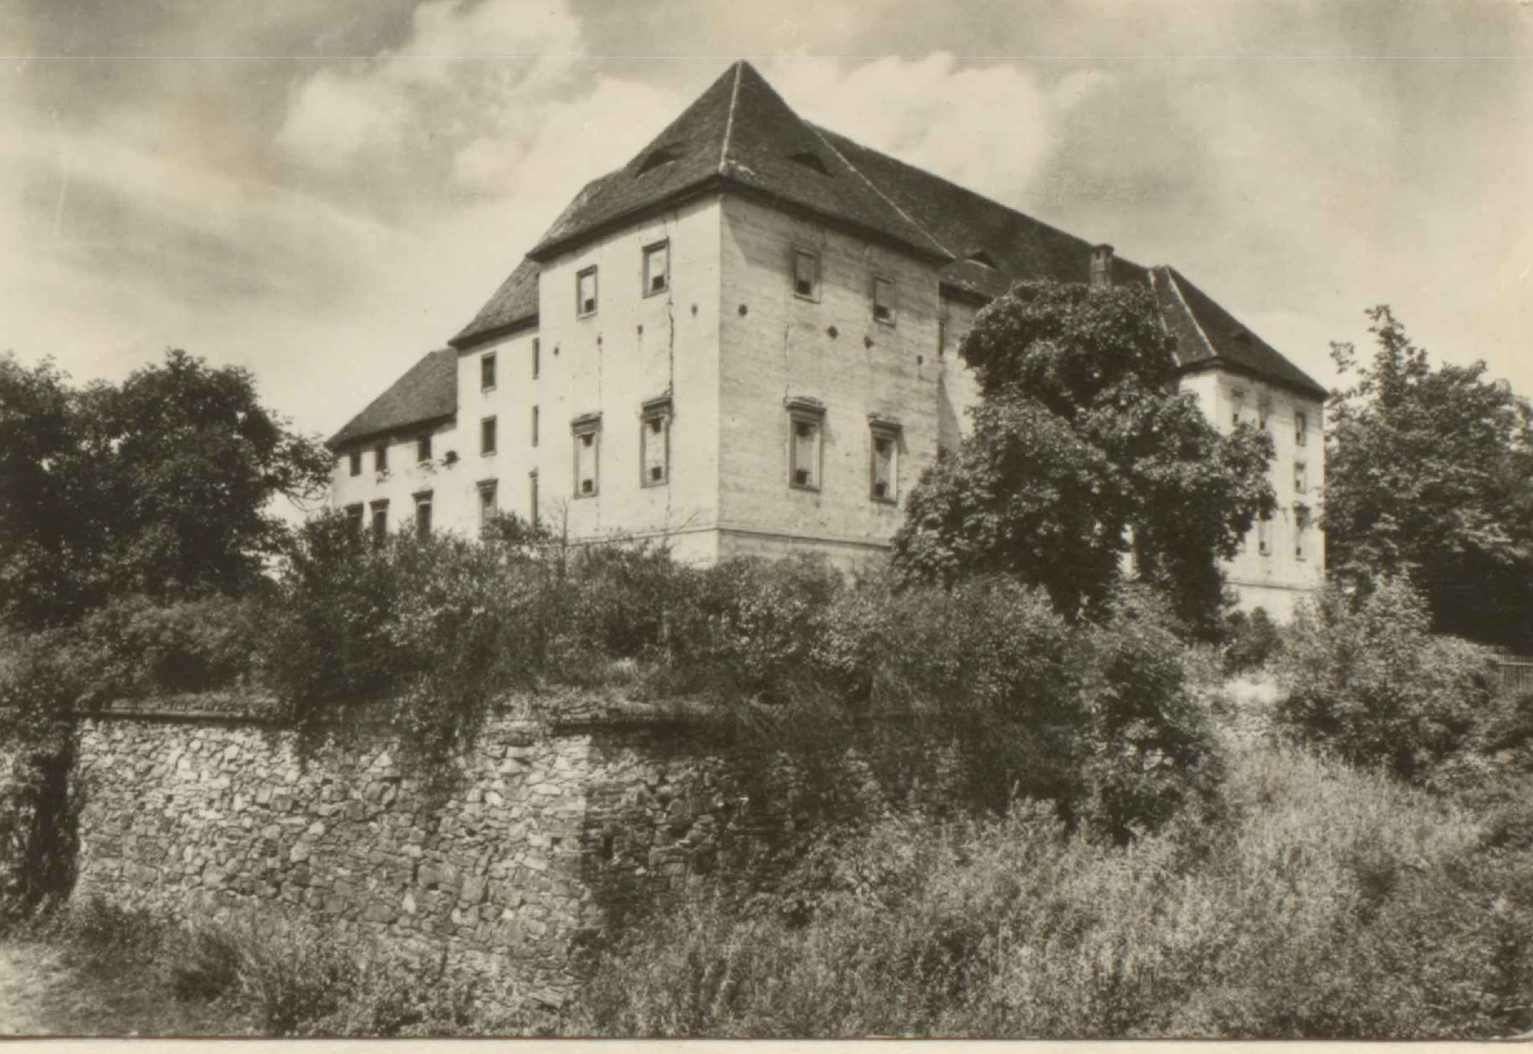
\includegraphics[width=\textwidth, height=\textheight, keepaspectratio]{017-a-zamek_kacerov}
\caption{Zámek Kaceřov, někdejší sídlo Gryspenů z Gryspachu
Sídla vrchnosti nad poddanými našimi předky}
\label{fig:017-a-zamek_kacerov}
\end{figure}

\begin{figure}
\centering
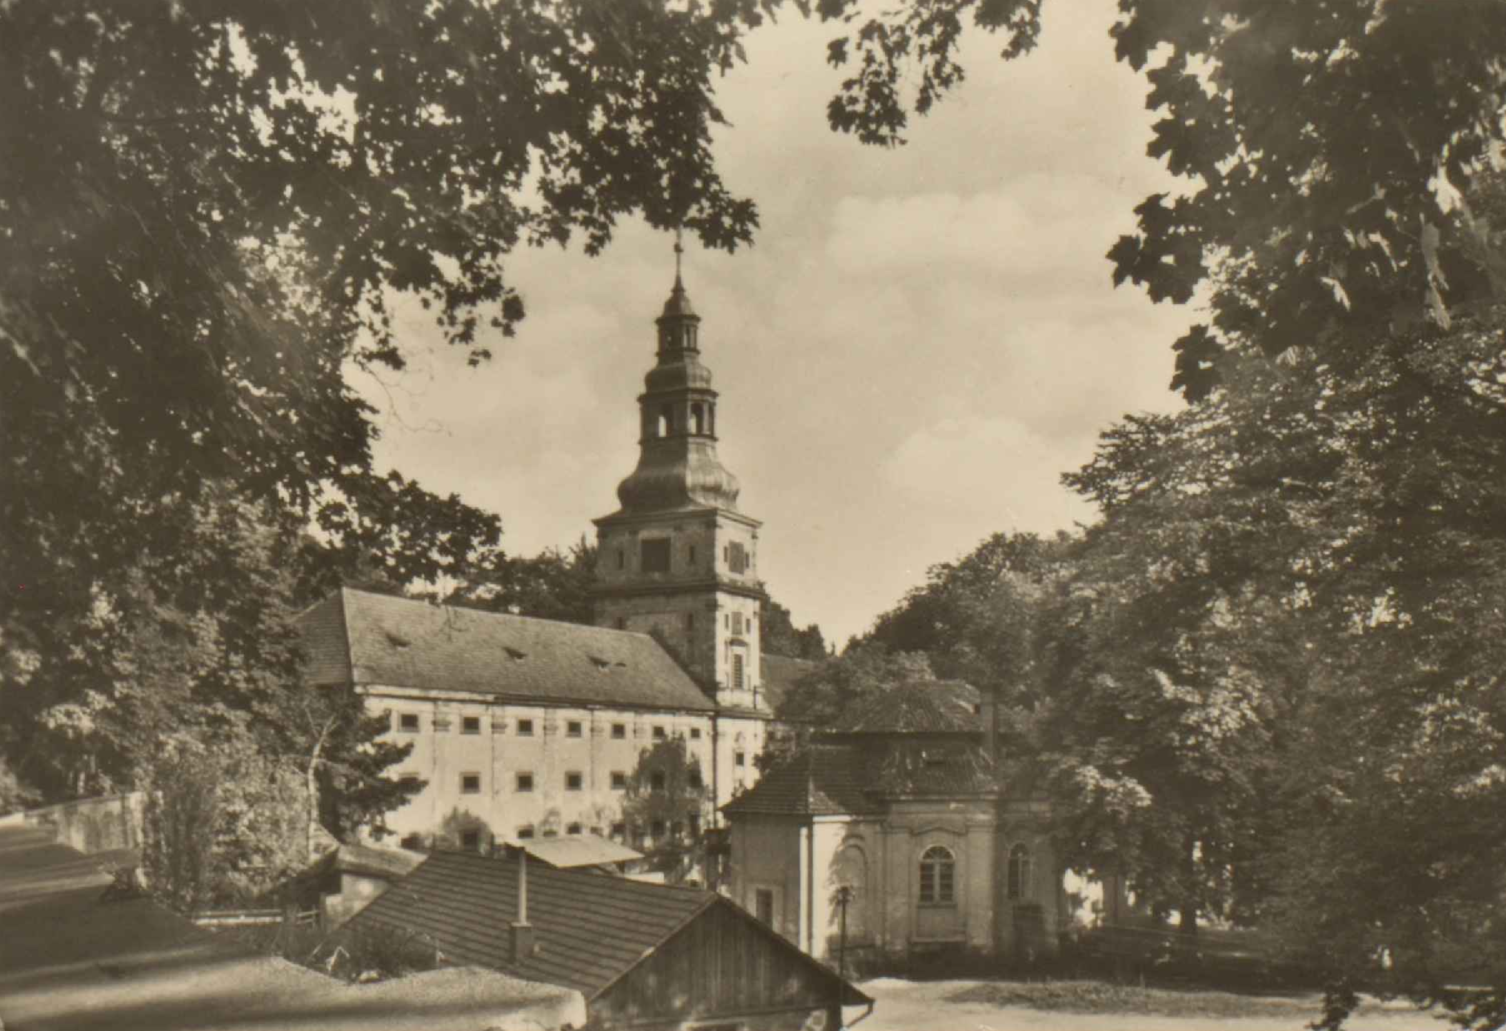
\includegraphics[width=\textwidth, height=\textheight, keepaspectratio]{017-b-sidlo_klastera}
\caption{Plasy, sídlo slavného kláštera a knížete Metternicha}
\label{fig:017-b-sidlo_klastera}
\end{figure}

% str 11 @ 18
\section{Prusíci narození v Sedlci}

% TODO tabulka

% str 12 @ 19
\section{Plasy a náš rod}
V půvabném údolí říčky Střely leží Plasy. Kníže Vladislav II. povolal sem v roce 1144 z kláštera Langheimského v Bavořích devět řeholníků cisterciácké­ho řádu a dal jim po otci svém zděděný dvůr Plasy se vším příslušenstvím. Postupem staletí vzmáhal se klášter i obec, takže před husitskou dobou patřil klášter plasský mezi největší v Čechách. Začátkem XVIII. století měl rozsáhlý majetek v celém kraji. V klášte­ře se zaměstnal veliký počet řemeslníků a umělců. Zvláště na růžích ustláno měli stavitelé, zedníci, truhláři, řezbáři, malíři i sochaři.

Před rokem 1700 dostal se jediný Prusík ze Sedlice a to Bartoloměj do Dřevce. Ten ovšem opustil již tu­to vesničku v roce 1627 a utekl do ciziny. Do konce XVII. století žili pak, jak je prokázáno Soupisem pod­daných podle víry po třicetileté válce, lidé s naším jménem jen v Sedlci. A tu kolem roku 1700 nebo krát­ce potom, objevuje se první Prusík jinde. V Plasích. Byl to Václav Prusík narozený 1678 v Sedlci.

Václav Prusík se domohl po nějakém čase hostinské živnosti a 1. října 1713 oženil se se Sabinou Kirchgangovou. Její otec byl Němec Simon Kirchgang, kovář v klášteře. Sabina se narodila rovněž jako její muž v roce 1678. Tento Václav Prusík byl prvním členem našeho rodu, který pojal za ženu Němku. Od roku 1713 vnikají tudíž i německé prvky do našeho rodu, který původně byl zcela slovanský. Václav zemřel 28. listopa­du 1728 v blízkých Nebřežinech a bylo mu tedy jen 50 let. Jeho žena Sabina přežila ho o 24 let a zemřela v roce 1752 v Plasích.

Václav měl dva syny a také dcery, ale ze všech zachoval se pouze jeden syn Eugenius Prusík. Dostal své jméno po tehdejším slavném opatovi kláštera Eugeniovi Tittlovi, který dokončil honosnou stavbu konventu. Eugenius narodil se 18. února 1714. Za manželku vzal si Češku Markétu Beránkovou, narozenou v Plasích v roce 1720. Eugenius Prusík velmi zručně maloval a byl i dobrým sta­vitelem. V roce 1780 přestavěl kostel sv. Vavřince v Kožlanech. Měl několik dětí. Dcera Luitgarda a syn Evžen zemřeli brzy, dcera Anna dožila se 14 let. Jediný jeho syn Adam dospěl. Eugenius Prusík zemřel v Plasích brzy po zrušení kláštera císařem Josefem II. a to 7. prosince 1786. Zažil největší rozkvět kláštera. Jeho žena Markéta pře­žila ho a zemřela ve věku 78 let v Plasích 26. října 1802.

Adam  Prusík, jediný potomek Eugenia, narodil se 30. července 1765. Když mu bylo 20 let, zašla sláva kláštera a nemohl již proto nabídnouti, jako vyučený zedník, své služby klášteru.

% str 12+1 @ 20

\begin{figure}
\centering
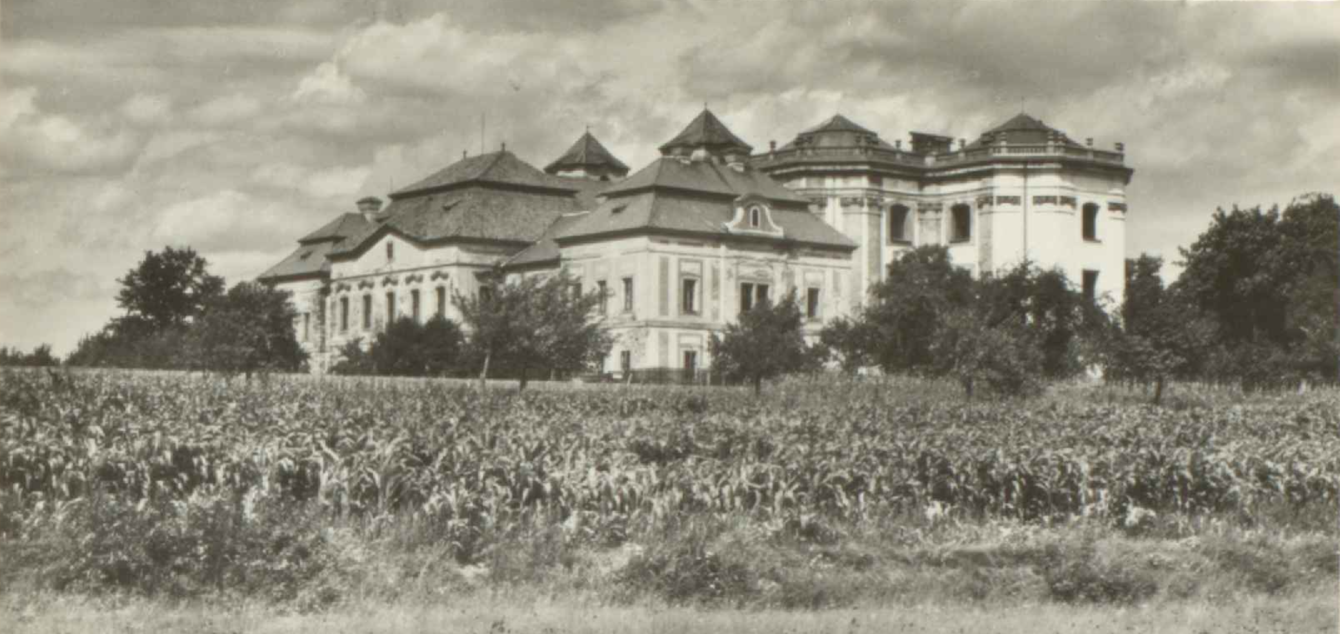
\includegraphics[width=\textwidth, height=\textheight, keepaspectratio]{020-a-marianska_tynice}
\caption{Mariánská Týnice u Kralovic, kterou pomáhal stavět Eugenius Prusík z Plas}
\label{fig:020-a-marianska_tynice}
\end{figure}
\begin{figure}
\centering
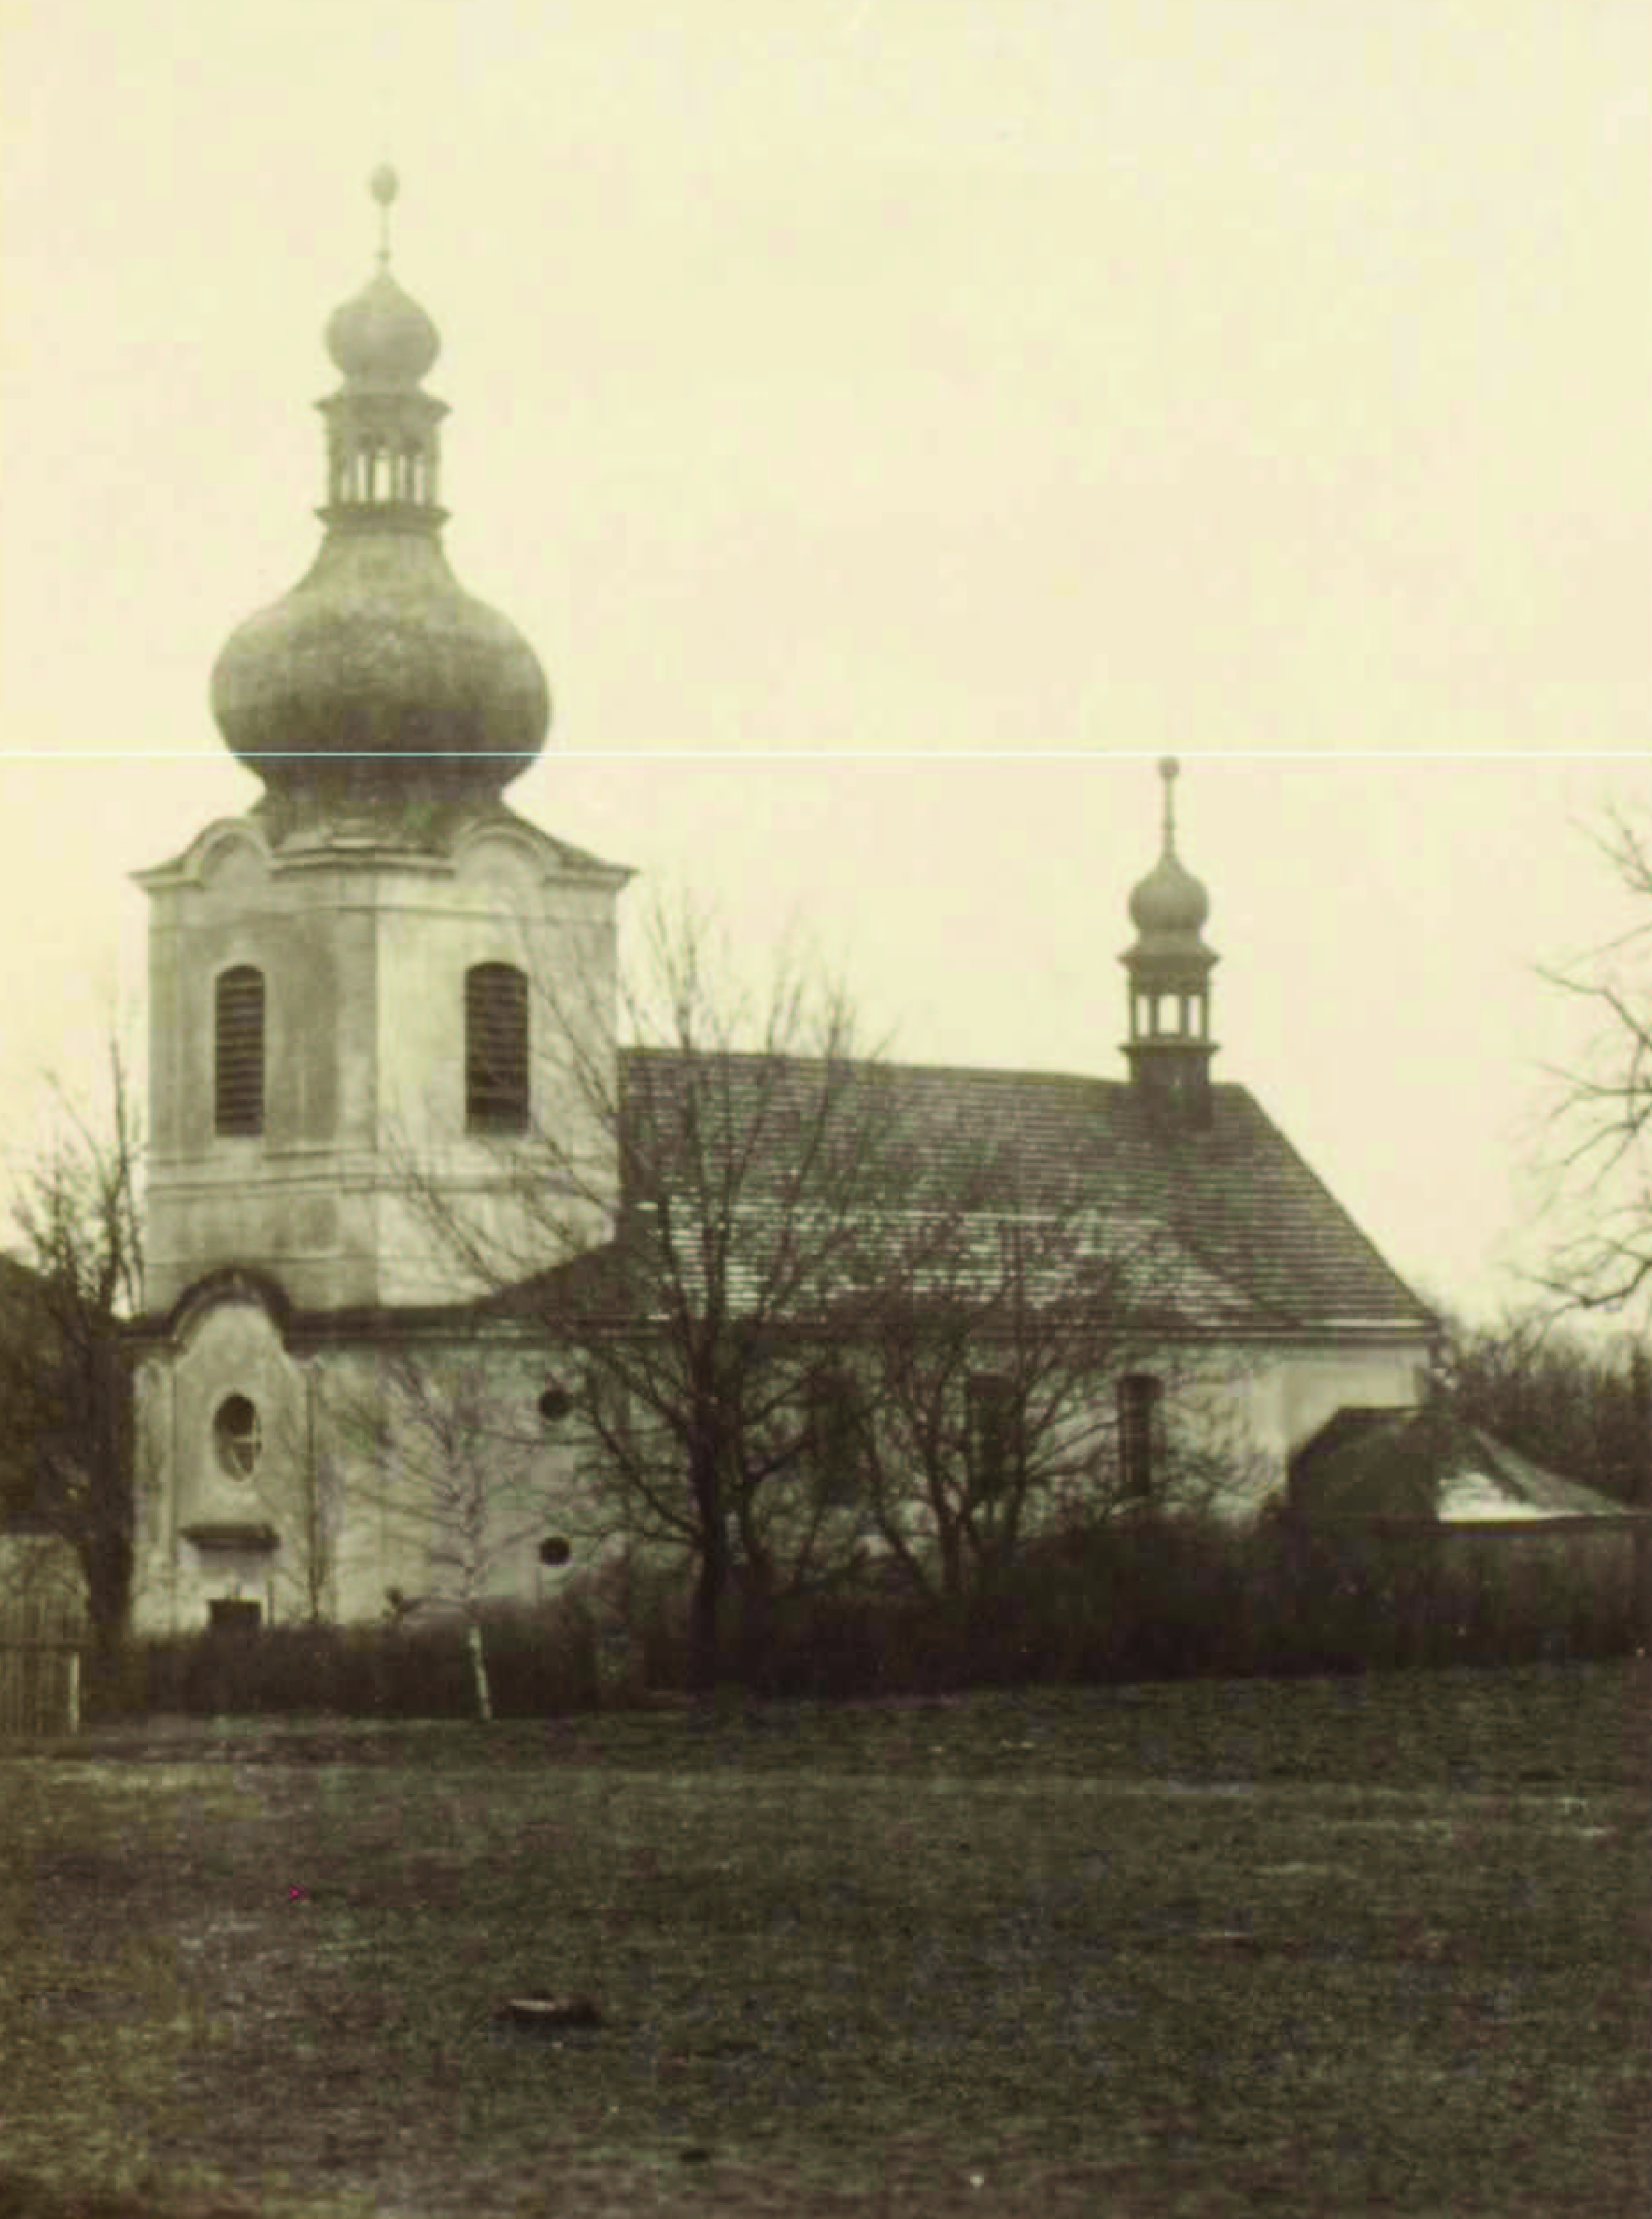
\includegraphics[width=\textwidth, height=\textheight, keepaspectratio]{020-b-kostel_svateho_vavrince}
\caption{Kostel svatého Vavřince v Kožlanech, přestavěl 1770 Eug. Prusík z Plas}
\label{fig:020-b-kostel_svateho_vavrince}
\end{figure}
\begin{figure}
\centering
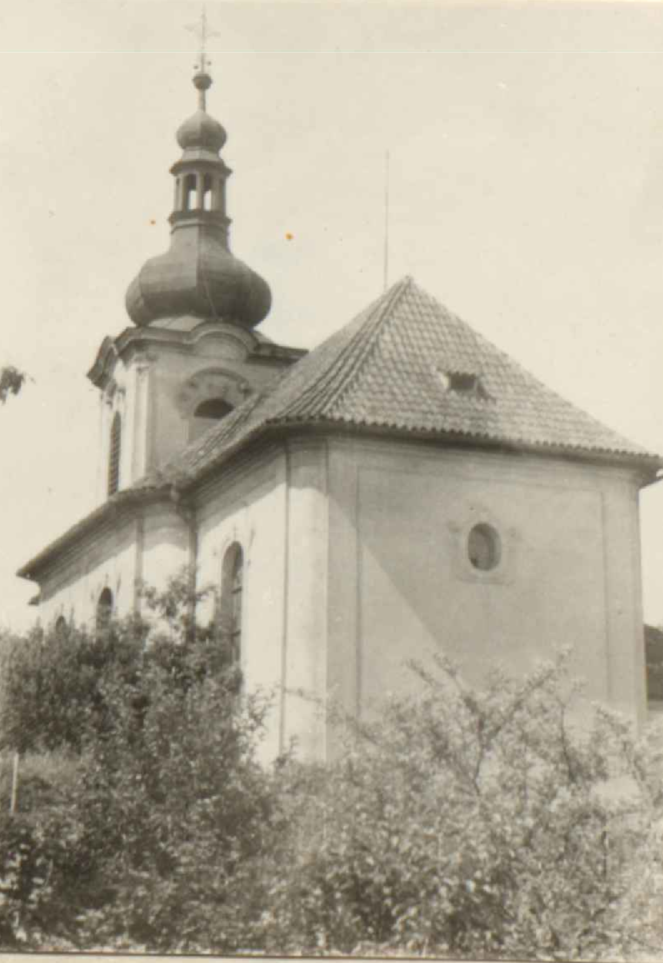
\includegraphics[width=\textwidth, height=\textheight, keepaspectratio]{020-c-kostel_svateho_klimenta}
\caption{Kostel svatého Klimenta v Chlumčanech u Loun roku 1776 vystavěl Martin Prusík z Plas}
\label{fig:020-c-kostel_svateho_klimenta}
\end{figure}

% str 13 @ 21
Oženil se 25. května 1789 s Rosalií Lohwasserovou, dcerou Němce, hajného z Velké Černé Hati. Novomanželé usadili se v blízké, malé, romaticky položené vesničce nad říčkou Střelou, Stražišti. Rosalie narodila se v roce 1764, ale není známo kdy a kde zemřela. Nestalo se tak ve Stražišti a dokončila svůj život někde u svých dětí. Adam jako zednický mistr byl velmi činný v blízkých vesnicích a ještě dodnes jsou v okolí stopy jeho stavitelské činnosti. V Chrašťovicích stojí někdejší sýpka, dnes obytné stavení a nad dveřmi je vytesáno jeho jméno a datum. Adam Prusík míval ve Stražišti i malý hostinec. Zemřel tam 2. září 1835.

Adam Prusík, usazený ve Stražišti, měl čtyři syny, kteří dospěli. Nejstarší z nich byl Vojtěch Prusík. Narodil se 22. dubna 1790, byl také mistrem zednickým. Se svou manželkou Annou Sieberovou z~blízkého Kalce, Němkou, měl řadu dětí. Vojtěch zemřel 24. července 1867 na marasmus. Je zakladatelem tzv. větve "Stražiště" a povíme si o něm obšírně a také o všech jeho potomcích, později.

Druhým synem Adamovým byl Josef Prusík. Vyučil se pivovarskému řemeslu a později usadil se v Jihlavě. Narodil se ve Stražišti 11. září 1792 a zemřel jako nejstarší z bratrů 12. června 1881. Za manželku měl Annu roz. Frűhaufovou z tehdy německé Jihlavy. Josef založil tzv. větev "Jihlava". Členové její se úplně poněmčili a věnujeme jim zvláštní kapitolu.

Třetím synem byl Jan Prusík. Narodil se 11. listopadu 1794 ve Stražišti a na přímluvu své­ho děda Lohwassera stal se nakonec lesníkem. Žil ve východních Čechách a na Vysočině a tam také mu pytlák násilně přetrhl nit života 21. března 1859. Stalo se to v rozsáhlých lesích u Svratky. Manžel­kou jeho byla Anna roz. Anderlová z Košumberku. Jan je zakladatelem větve tzv. "Kuchyně u Herálce". Život jeho a potomků vylíčíme později.

Čtvrtým synem Adamovým byl Václav Prusík. Narodil se 24. února 1797 ve Stražišti. Stal se také hajným, ale v mladém věku, svobodný, zemřel 28. ledna 1827 ve svém rodišti.

% str 14 @ 22
Syn sedláka Adama Prusíka v Sedlci, Martin Prusík, měl při svém zrození 9. ledna 1745 již příbuzné v Plasích. Pro tehdejší dobu a kraj byly Plasy tenkrát něco podobného jako v pozdějších dobách Praha nebo Vídeň se svými velkými pracovními příležitostmi. Martina nedali na sedlačinu, ale na zedničinu. Byl to velmi chytrý chlapec a brzy se stal zednickým mistrem v Plasích. Učil se u svého strýce Eugenia Prusíka a nepůsobil jen zde, ale i v krajích vzdálenějších. Ví se o něm, že stavěl řadu kostelů, ale bohužel doklady jsou jen pro stavbu kostela sv. Klimenta v Chlumčanech u Loun v roce 1771. Když se kdysi hle­dalo, jak skutečně ve své plné slávě vypadal hrad Krašov, našla se náhodou kresba tohoto kdysi mocné­ho hradu, podepsaná Martinem Prusíkem z Plas. Jsou však zachovány i jiné jeho kresby, a to dvora Hubenova nebo zámku Kaceřova.

Když přebíral Martinův bratr Blažej rodný grunt v Sedlci, oženil se Martin Prusík. Stalo se to 10.~října 1776 a jeho nevěsta Kateřina Kaplánková nepocházela přímo z kraje, jak si tehdy ženiši své ženy vyhledá­vali, ale až z Radnic. I to svědčí o tom, že Martin jako stavitel hojně cestoval po Čechách a zvláště v mladých letech zdaleka nebyly Plasy jeho jediným působištěm. Kateřina narodila se v roce 1748 a manželé poměrně pozdě měli své děti. Nejstarší byla dcera Alžběta, která se narodila v roce 1780 a vdala se za panského kováře Kabáta v Plasích. Další jejich dcera Barbora narodila se v roce 1792 a zemřela svobodná 15. srpna 1865 v Plasích. V matrice zemřelých je uvede­no, že byla žebračka. Podivné jsou osudy lidí! Je­jí rodiče byli vážení občané v Plasích a dcera umírá sama a v nouzi! Martin Prusík měl ještě řadu dětí, které brzy zemřely, ale také tři syny, kteří dospěli. Sám zemřel 30. října 1822 ve věku 82 let. Jeho žena Kateřina zemřela 20. července 1835.

Nejstarším synem Martinovým, který dospěl, byl Josef Prusík, narodil se 1781, ale brzy svobodný zemřel.

Dalším synem byl František Prusík, který se narodil v Plasích 22. srpna 1789. U otce vyučil se zednickému řemeslu a usadil se později v Nebřežinech. Za ženu měl Josefu Gűtterovou z Nebřežin. Tam se jim narodily 2 děti, ale brzy se všichni odstěhovali do Červené Řečice u Pelhřimova, kde František dostal dobré místo jako zednický mistr na arcibiskupském zámku. V Červené Řečici také František zemřel 28. srpna 1838. Po něm dnes již zcela vymřelá větev je nazvána tzv. "Červená Řečíce". Její osudy ještě vylíčíme.

% str 15 @ 23
Třetím synem byl zase Josef Prusík. Narodil se 20. března 1796 a nechtěl býti po otci zedníkem. Brzy se přiženil k dceři obuvníka Janě Říhové do Nebřežin a tam se také vyučil tomuto řemeslu a již tam do smrti zůstal. Měli spolu deset dětí a budeme o nich vyprávěti. Josef zemřel ve věku 79 let 9. ledna 1875 v Nebřežinech u Plas. Je zakladatelem tzv. větve "Nebřežiny".

Posledním synem byl Antonín Prusík. Narodil se 21. ledna 1799 v Plasích. I on stal se zedníkem jako jeho otec Martin, ale dlouho byl pak na vojně. Za manželku měl dceru prvního českého učitele v Plasích Josefu Dűrschmiedovou. Je zakladatelem tzv. větve "Plasy". Zmíníme se o všech je­ho potomcích v dalších kapitolách.

První členové rodu, kteří přišli ze Sedlce do Plas začátkem 18. století, jako byl Václav a pak opět Martin v druhé polovině 18. století, stali se svý­mi potomky budovateli dalších rodových větví. Proto jsou Plasy vedle Sedlce významným historickým místem pro nás.

\section{Ze Sedlce do Výrova}
Třetím Prusíkem, nepočítáme-li Bartoloměje, který opustil domov již v první polovině XVII. století a usadil se nakrátko ve Dřevci, byl první syn rychtáře Blažeje Prusíka Vojtěch, který také opustil domov. Na gruntě v Sedlci zůstal jeho mladší bratr Václav. Vojtěch Prusík narodil se 31. března 1777 za Marie Terezie. Oba bratři seznámili se se svými ženami - sestrami z Výrova č. 18. Svatbu sla­vili společně 8. října 1803. Bylo to v době slávy Napoleonovy. Vojtěch Prusík, který se stal rychtářem ve Výrově u Královic, je budovatelem naší nejsilnější rodové větve tzv. "Výrov". Budeme o ní obšírně vyprá­vět.

% str 16 @ 24
\section{Rodové větve}
V předešlých kapitolách o Sedlci a Plasích vylí­čili jsme již krátce život zakladatelů, osmi rodo­vých větví. Devátá větev tzv. "Polská" tvoří zcela zvláštní kapitolu, neboť jedná se o veliký po­čet potomků českého exulanta Bartoloměje Prusíka pobělohorské doby. Tito lidé nežijí dnes jen v Polsku, ale i daleko za mořem. A zdá se, že v Polsku nejde jen o rodovou větev!

Pro úplný obraz rodu, jak se dnes po tolika staletích jeví, zachycujeme na věčnou paměť všechny jejich po­tomky, pokud se dožili alespoň deseti let. Nejde tedy jen o tzv. "meč", ale i "přeslici". Zakladatelé našich rodových větví rodili se v pohnutých dobách francouzské revoluce a napoleonských válek. Všech osm Prusíků - zakladatelů narodilo se v průběhu let 1777 – 1799. Snad bude se zdáti někdy i únavné pročítati všechna jména i životy několika tisíc potomků, ale bez toho nebyl by profil našeho rodu dostatečný. Do potomků po přeslici a tedy nejen po meči, patří mnozí  významní lidé, často s pestrými osudy, nemající sice již jméno Prusík, ale přece jen naši krev. Je to dodnes přes 670 jiných jmen.

\textbf{Zakladatelé}
% TODO seznam

% str 17 @ 25
\section{Několik charakteristik}
Kraj, v němž žili naši předci, patřil od pradávna do kraje Rakovnického. Také Soupis poddaných podle víry, dokončený v dubnu 1651, patří do tohoto kraje, ačkoliv panstvím byli naši předci poddáni Plasům a potom i jiným vrchnostem. A tyto vrchnosti nesídlily vždy v Rakovnickém kraji. Teprve 21. srpna 1788, nedlouho před smrtí císařovny Marie Terezie, bylo celé Plassko začleněno do Plzeňského kraje. Všechny katastrální zápisy a berní povinnosti jsou od toho dne vedeny již v tomto kraji, kam jistě Sedlec etnograficky vždy spíše patřil. Když mluvíme o povinnostech poddaných, tu jistě nás musí zaraziti to, že v době Gryspeků v 16. století prakticky nebylo robot a jen vlastně platilo se vrchnosti buď naturáliemi, nebo penězi. I v mnohem pozdějších staletích představoval nájem pro sedláky různý druh berních povinností. Žilo se tehdy leckdy poměrně snadno a jindy zase byl život velmi krutý.

V 18. až 19. století byla již robota zcela vžitým pojmem. Sedlák měl robotní povinnost s potahem, a to celý rok týdně s dvěma kusy tři dny, ale protože vždy celý den neobětoval, musil ještě tři dny ruční roboty posílati. Když byly v týdnu dva svátky, robota byla jen dva dny. O vánocích a velikonocích byl týden bez roboty. Ve žních dostávala robotující osoba bochníček chleba a dvakrát denně jídlo. Za celé žně dostali pak poddaní v jedné obci celou várku piva o osmnácti sudech čtyřvědrových. Chalupníci robotovali ručně tři dny, někteří z nich jen dva dny.

Obilí na prodej se vozívalo z celého Plasska do Mantiny, jak se říkalo Manětínu a někdy též do Mlác, jak se říkalo Mladoticům. Tam obilí kupoval hostinsky. Někdy také přijížděli pro obilí sami formani. Do Bílova formani jezdili málo, poněvadž si stěžovali, že v obilí bývá "stoklas". V Sedlici bývalo obilí dobré kvality.

Ve vesnicích menších nebývalo vždy mnoho řemeslníků v dávných dobách. Tak v Sedlci byl kovář, ale krejčí jen v blízké Žebnici, krčmáři byli v Plasích, Mladoticích, Dřevci, Hrádecku nebo v Královicích, ševci také jinde, šindelář v Kopidle, kameník v Potvorově, tkadlec v Černíkovicích a na Hadačce, ovčácký mistr jen v Plasích, Sechuticích a v Královicích. Mlynářů bylo však hojnost.

% str 18 @ 26
Za panování císaře Rudolfa II. kolem roku 1600 žili Prusíci jen v jednom místě, v Sedlci. Tak to bylo i po třicetileté válce v Čechách, ale mimo to již tehdy žil jeden člen rodu v Polsku. V době tureckých válek po roce 1700 žili Prusíci v Čechách již na dvou místech, v Sedlci a v Plasích. V době Napoleonově, kolem roku 1800, žili již i ve Stražišti. Po revolučním roce 1848 existovali členo­vé našeho rodu již na třinácti místech v Čechách. A v roce 1968, kdy píšeme tyto dějiny našeho rodu, žijí členové v naší vlasti a ve světě nejméně ve čtyřech stech různých místech.

Dnes se tvrdí, že se věk lidí prodlužuje proti minulosti. Je pravdou, že úmrtnost dětí byla kdysi obrovská. Často v rodinách s deseti až patnácti dětmi dospěly jen dvě. Je pravda, že mnoho zhoubných nemo­cí, jako byly černé neštovice a záškrt, byly vymýceny, zrovna tak jako úmrtnost rodiček. Když však sledujeme věk našich dávných předků, jeví se to vše v poněkud jiném světle. Byly války, těžké doby, robota, ale život měl v celku pomalejší a klidnější tempo, bylo méně hřmotu, risika a všeho toho špatného, co nám zase přinesla nová doba a civilizace. I tento jiný ráz života našich předků přispěl asi k tomu faktu, že průměrný věk osmnácti Prusíků, narozených v~Sedlci od roku 1515 až do roku 1825 je 65 let.

Pozoruhodné je, jak některé pozdější rodové větve jsou početné a jiné velmi malé a jak také se měnila národnost jejích členů. Je pravda, že ve všech větvích jsou zaznamenáni členové, kteří žili nebo žijí dnes v cizině. Mnozí z nich však ztratili národnost teprve emigrací za oceán, do Vídně a jinam, ale někteří již také přímo v Čechách.

Nejsilnější naší rodovou větví je tzv. "Výrov". Pátrání po potomcích a jejích členech bylo sice obtížné, ale nejúspěšnější. Početnost její lze si vysvětlit také tím, že její zakladatel Vojtěch Prusík měl osm dětí a z nich jen syn Blažej byl knězem. Další tři synové a čtyři dcery měli četné potomky. Není tomu tak již v jiných větvích.

Větev "Sedlec" je sice dosti silná proti ostatním, ale přece jen o dvě třetiny slabší než výrovská. Její za­kladatel Václav Prusík, bratr Vojtěchův, měl sice šest dětí, které dospěly aspoň deseti let, ale dcera Barbora, provdaná Levá, zůstala bezdětná, další Marie zemřela jako desetileté děvče a jen Kateřina, provdaná Kouklová, měla četné potomky.
% str 19 @ 27
Syn František zemřel ve 21 letech a měl pouze jednu dcerku, Tomáš se dožil jen čtyřiceti let a jen Vojtěch měl četnější potomky.

Větev "Červená Řečíce", jejímž zakladatelem byl František Prusík, je vůbec nejslabší a dnes je již tato větev úplně uschlá.

U větve "Nebřežiny", jejímž zakladatelem byl Josef Prusík, je mezera u potomků jeho dcery Josefy, provdané Křížové v Nebřežinech. Je to průměrně silná větev.

Větev "Plasy" založil Antonín Prusík a je to malá větev.

Dosti velký počet potomků se poněmčil nebo jinak ztratil českou národnost z větve "Stražiště". Zakladatelem jejím je Vojtěch Prusík.

Úplně poněmčená je větev tzv. "Jihlava", jejímž zakladatelem byl Josef Prusík. Nebyla kdysi nejmenší, ale dnes žije již velmi málo jejích členů a to jen v Rakousku a Německu.

Větev tzv. "Kuchyně u Herálce", kde v myslivně působil a zemřel její zakladatel Jan Prusík, je průměrně silná. Také někteří její členové ztratili českou národ­nost.

Snad se může po letech státi, že některá naše další větev vymře, ale jejím zánikem určitě nezmizí náš rod. Vždyť po meči žijí nás stovky a po přeslici jsou to tisíce. Nyní vylíčíme podrobně osudy všech rodových větví. Bude to od roku 1805, kdy se narodilo první dítě nejstaršímu ze zakladatelů větví Vojtěchu Prusíkovi ve Výrově až po naše časy do roku 1968, kdy sepisujeme tyto dějiny našeho rodu.

% str 19+1 @ 28

\begin{figure}
\centering
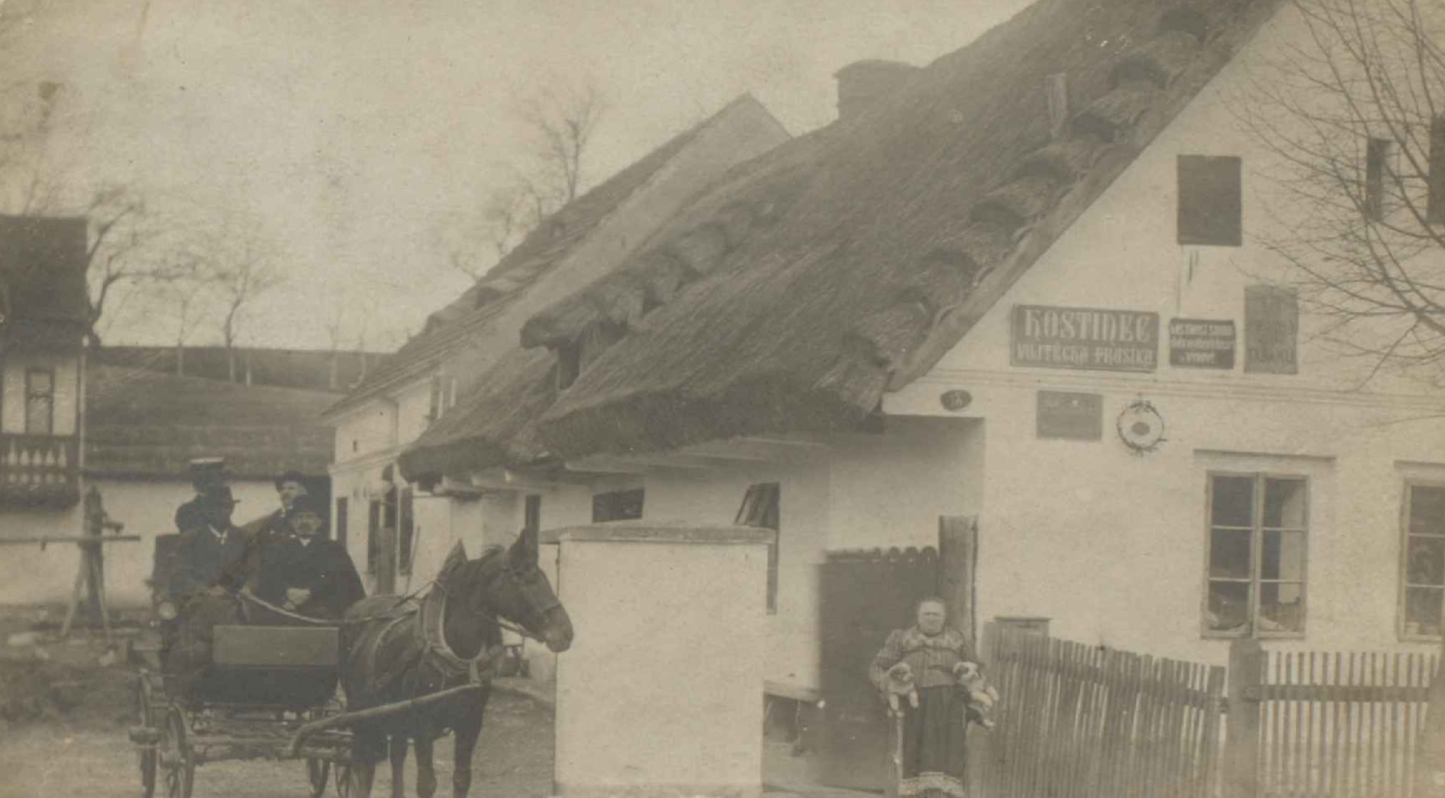
\includegraphics[width=\textwidth, height=\textheight, keepaspectratio]{028-a-statek_c_18_ve_vyrove}
\caption{Statek číslo 8 ve Výrově „u Boudů“, kam se roku 1803 přiženil Vojtěch Prusík ze Sedlice a založil zde rozsáhlou větev rodu. Snímek z roku 1808}
\label{fig:028-a-statek_c_18_ve_vyrove}
\end{figure}

\begin{figure}
\centering
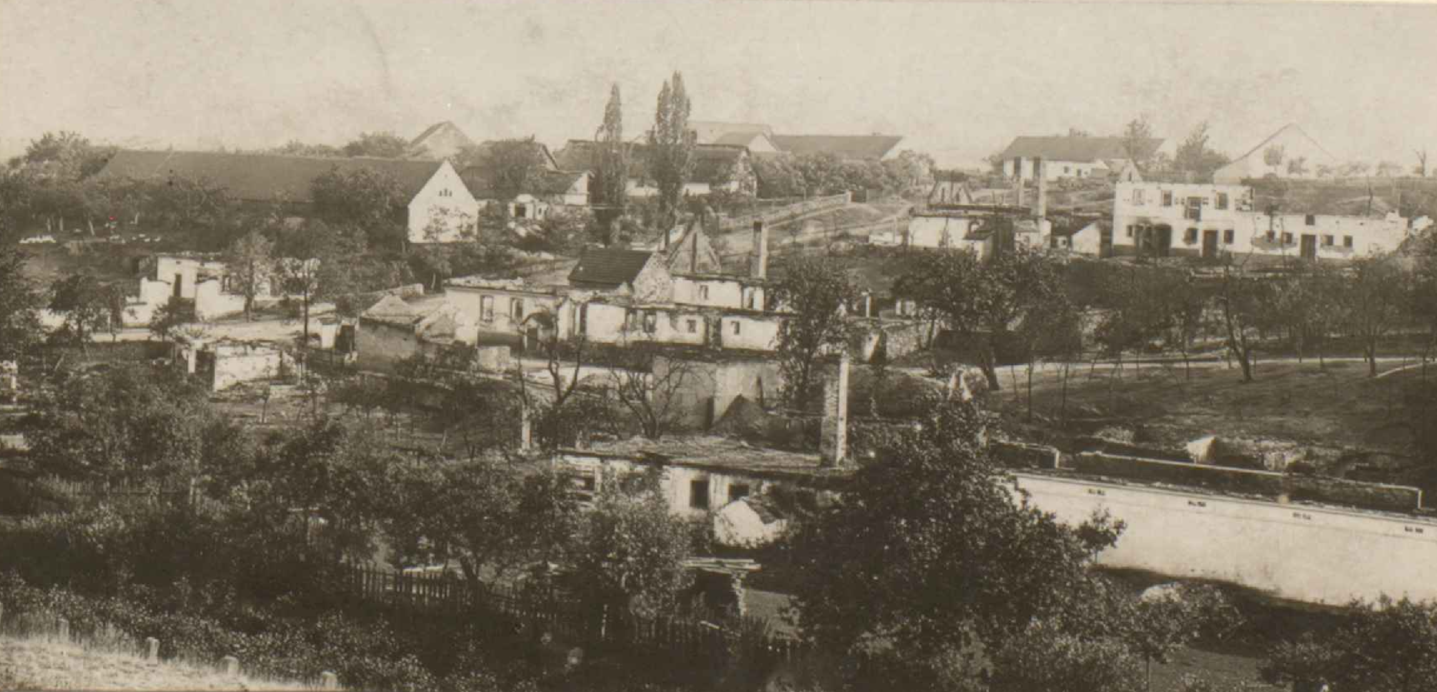
\includegraphics[width=\textwidth, height=\textheight, keepaspectratio]{028-b-pohled_na_vyrov}
\caption{Pohled na Výrov po požáru v roce 1911}
\label{fig:028-b-pohled_na_vyrov}
\end{figure}


\end{document}
